% Options for packages loaded elsewhere
\PassOptionsToPackage{unicode}{hyperref}
\PassOptionsToPackage{hyphens}{url}
%
\documentclass[
  ignorenonframetext,
]{beamer}
\usepackage{pgfpages}
\setbeamertemplate{caption}[numbered]
\setbeamertemplate{caption label separator}{: }
\setbeamercolor{caption name}{fg=normal text.fg}
\beamertemplatenavigationsymbolsempty
% Prevent slide breaks in the middle of a paragraph
\widowpenalties 1 10000
\raggedbottom
\setbeamertemplate{part page}{
  \centering
  \begin{beamercolorbox}[sep=16pt,center]{part title}
    \usebeamerfont{part title}\insertpart\par
  \end{beamercolorbox}
}
\setbeamertemplate{section page}{
  \centering
  \begin{beamercolorbox}[sep=12pt,center]{part title}
    \usebeamerfont{section title}\insertsection\par
  \end{beamercolorbox}
}
\setbeamertemplate{subsection page}{
  \centering
  \begin{beamercolorbox}[sep=8pt,center]{part title}
    \usebeamerfont{subsection title}\insertsubsection\par
  \end{beamercolorbox}
}
\AtBeginPart{
  \frame{\partpage}
}
\AtBeginSection{
  \ifbibliography
  \else
    \frame{\sectionpage}
  \fi
}
\AtBeginSubsection{
  \frame{\subsectionpage}
}
\usepackage{amsmath,amssymb}
\usepackage{iftex}
\ifPDFTeX
  \usepackage[T1]{fontenc}
  \usepackage[utf8]{inputenc}
  \usepackage{textcomp} % provide euro and other symbols
\else % if luatex or xetex
  \usepackage{unicode-math} % this also loads fontspec
  \defaultfontfeatures{Scale=MatchLowercase}
  \defaultfontfeatures[\rmfamily]{Ligatures=TeX,Scale=1}
\fi
\usepackage{lmodern}
\usetheme[]{Madrid}
\ifPDFTeX\else
  % xetex/luatex font selection
\fi
% Use upquote if available, for straight quotes in verbatim environments
\IfFileExists{upquote.sty}{\usepackage{upquote}}{}
\IfFileExists{microtype.sty}{% use microtype if available
  \usepackage[]{microtype}
  \UseMicrotypeSet[protrusion]{basicmath} % disable protrusion for tt fonts
}{}
\makeatletter
\@ifundefined{KOMAClassName}{% if non-KOMA class
  \IfFileExists{parskip.sty}{%
    \usepackage{parskip}
  }{% else
    \setlength{\parindent}{0pt}
    \setlength{\parskip}{6pt plus 2pt minus 1pt}}
}{% if KOMA class
  \KOMAoptions{parskip=half}}
\makeatother
\usepackage{xcolor}
\newif\ifbibliography
\usepackage{color}
\usepackage{fancyvrb}
\newcommand{\VerbBar}{|}
\newcommand{\VERB}{\Verb[commandchars=\\\{\}]}
\DefineVerbatimEnvironment{Highlighting}{Verbatim}{commandchars=\\\{\}}
% Add ',fontsize=\small' for more characters per line
\usepackage{framed}
\definecolor{shadecolor}{RGB}{248,248,248}
\newenvironment{Shaded}{\begin{snugshade}}{\end{snugshade}}
\newcommand{\AlertTok}[1]{\textcolor[rgb]{0.94,0.16,0.16}{#1}}
\newcommand{\AnnotationTok}[1]{\textcolor[rgb]{0.56,0.35,0.01}{\textbf{\textit{#1}}}}
\newcommand{\AttributeTok}[1]{\textcolor[rgb]{0.13,0.29,0.53}{#1}}
\newcommand{\BaseNTok}[1]{\textcolor[rgb]{0.00,0.00,0.81}{#1}}
\newcommand{\BuiltInTok}[1]{#1}
\newcommand{\CharTok}[1]{\textcolor[rgb]{0.31,0.60,0.02}{#1}}
\newcommand{\CommentTok}[1]{\textcolor[rgb]{0.56,0.35,0.01}{\textit{#1}}}
\newcommand{\CommentVarTok}[1]{\textcolor[rgb]{0.56,0.35,0.01}{\textbf{\textit{#1}}}}
\newcommand{\ConstantTok}[1]{\textcolor[rgb]{0.56,0.35,0.01}{#1}}
\newcommand{\ControlFlowTok}[1]{\textcolor[rgb]{0.13,0.29,0.53}{\textbf{#1}}}
\newcommand{\DataTypeTok}[1]{\textcolor[rgb]{0.13,0.29,0.53}{#1}}
\newcommand{\DecValTok}[1]{\textcolor[rgb]{0.00,0.00,0.81}{#1}}
\newcommand{\DocumentationTok}[1]{\textcolor[rgb]{0.56,0.35,0.01}{\textbf{\textit{#1}}}}
\newcommand{\ErrorTok}[1]{\textcolor[rgb]{0.64,0.00,0.00}{\textbf{#1}}}
\newcommand{\ExtensionTok}[1]{#1}
\newcommand{\FloatTok}[1]{\textcolor[rgb]{0.00,0.00,0.81}{#1}}
\newcommand{\FunctionTok}[1]{\textcolor[rgb]{0.13,0.29,0.53}{\textbf{#1}}}
\newcommand{\ImportTok}[1]{#1}
\newcommand{\InformationTok}[1]{\textcolor[rgb]{0.56,0.35,0.01}{\textbf{\textit{#1}}}}
\newcommand{\KeywordTok}[1]{\textcolor[rgb]{0.13,0.29,0.53}{\textbf{#1}}}
\newcommand{\NormalTok}[1]{#1}
\newcommand{\OperatorTok}[1]{\textcolor[rgb]{0.81,0.36,0.00}{\textbf{#1}}}
\newcommand{\OtherTok}[1]{\textcolor[rgb]{0.56,0.35,0.01}{#1}}
\newcommand{\PreprocessorTok}[1]{\textcolor[rgb]{0.56,0.35,0.01}{\textit{#1}}}
\newcommand{\RegionMarkerTok}[1]{#1}
\newcommand{\SpecialCharTok}[1]{\textcolor[rgb]{0.81,0.36,0.00}{\textbf{#1}}}
\newcommand{\SpecialStringTok}[1]{\textcolor[rgb]{0.31,0.60,0.02}{#1}}
\newcommand{\StringTok}[1]{\textcolor[rgb]{0.31,0.60,0.02}{#1}}
\newcommand{\VariableTok}[1]{\textcolor[rgb]{0.00,0.00,0.00}{#1}}
\newcommand{\VerbatimStringTok}[1]{\textcolor[rgb]{0.31,0.60,0.02}{#1}}
\newcommand{\WarningTok}[1]{\textcolor[rgb]{0.56,0.35,0.01}{\textbf{\textit{#1}}}}
\usepackage{graphicx}
\makeatletter
\def\maxwidth{\ifdim\Gin@nat@width>\linewidth\linewidth\else\Gin@nat@width\fi}
\def\maxheight{\ifdim\Gin@nat@height>\textheight\textheight\else\Gin@nat@height\fi}
\makeatother
% Scale images if necessary, so that they will not overflow the page
% margins by default, and it is still possible to overwrite the defaults
% using explicit options in \includegraphics[width, height, ...]{}
\setkeys{Gin}{width=\maxwidth,height=\maxheight,keepaspectratio}
% Set default figure placement to htbp
\makeatletter
\def\fps@figure{htbp}
\makeatother
\setlength{\emergencystretch}{3em} % prevent overfull lines
\providecommand{\tightlist}{%
  \setlength{\itemsep}{0pt}\setlength{\parskip}{0pt}}
\setcounter{secnumdepth}{-\maxdimen} % remove section numbering
\logo{
\includegraphics[height=1cm,width=3cm]{logo.png}}
\usetheme{Madrid}
\usefonttheme{serif}
\setbeamertemplate{navigation symbols}{}

\usepackage{amsmath}

\usepackage{graphicx}
\setkeys{Gin}{width=0.5\linewidth} 


\usepackage{booktabs}
\usepackage{longtable}
\usepackage{array}
\usepackage{multirow}
\usepackage{wrapfig}
\usepackage{float}
\usepackage{colortbl}
\usepackage{pdflscape}
\usepackage{tabu}
\usepackage{threeparttable}
\usepackage{threeparttablex}
\usepackage[normalem]{ulem}
\usepackage{makecell}
\usepackage{xcolor}
\ifLuaTeX
  \usepackage{selnolig}  % disable illegal ligatures
\fi
\usepackage{bookmark}
\IfFileExists{xurl.sty}{\usepackage{xurl}}{} % add URL line breaks if available
\urlstyle{same}
\hypersetup{
  pdftitle={Lecture 5},
  pdfauthor={Endri Raco},
  hidelinks,
  pdfcreator={LaTeX via pandoc}}

\title{Lecture 5}
\subtitle{Data Visualization with Python : Matplotlib}
\author{Endri Raco}
\date{05 March, 2025}

\begin{document}
\frame{\titlepage}

\begin{frame}[allowframebreaks]
  \tableofcontents[hideallsubsections]
\end{frame}
\section{Introduction}\label{introduction}

\begin{frame}{Using the matplotlib.pyplot interface}
\phantomsection\label{using-the-matplotlib.pyplot-interface}
There are many ways to use Matplotlib.

In this lecture, we will focus on the \textbf{pyplot} interface, which
provides the most flexibility in creating and customizing data
visualizations.
\end{frame}

\begin{frame}{Using the matplotlib.pyplot interface}
\phantomsection\label{using-the-matplotlib.pyplot-interface-1}
Initially, we will use the pyplot interface to create two kinds of
objects: Figure objects and Axes objects.

This lecture introduces a lot of new concepts, so if you ever need a
quick refresher, download the Matplotlib Cheat Sheet and keep it handy!
\end{frame}

\begin{frame}{Introduction to Google Colab}
\phantomsection\label{introduction-to-google-colab}
\begin{itemize}
\tightlist
\item
  Google Colab is a \textbf{cloud-based Jupyter Notebook} environment.
\item
  It allows you to write and run \textbf{Python code} without
  installation.
\item
  Colab provides \textbf{free access to GPUs and TPUs} for machine
  learning.
\item
  \textbf{No setup required}---just log in with a Google account.
\end{itemize}
\end{frame}

\begin{frame}{Key Features of Colab}
\phantomsection\label{key-features-of-colab}
\begin{itemize}
\tightlist
\item
  \textbf{Runs in the cloud} (no local setup needed).
\item
  \textbf{Supports Python 3} with pre-installed libraries.
\item
  \textbf{Free GPUs and TPUs} for deep learning.
\item
  \textbf{Collaborate in real-time} like Google Docs.
\item
  \textbf{Supports LaTeX, Markdown, and interactive widgets.}
\end{itemize}
\end{frame}

\begin{frame}{Opening Google Colab}
\phantomsection\label{opening-google-colab}
\begin{enumerate}
\tightlist
\item
  Go to \href{https://colab.research.google.com/}{Google Colab}.
\item
  Click \textbf{File → New Notebook}.
\item
  Start coding in the cells (Python code or Markdown text).
\end{enumerate}
\end{frame}

\begin{frame}[fragile]{Writing and Running Python Code}
\phantomsection\label{writing-and-running-python-code}
\AddToHookNext{env/Highlighting/begin}{\tiny}

\begin{Shaded}
\begin{Highlighting}[]
\CommentTok{\# Simple Python code in Colab}
\BuiltInTok{print}\NormalTok{(}\StringTok{"Hello, Google Colab!"}\NormalTok{)}
\end{Highlighting}
\end{Shaded}

\begin{itemize}
\tightlist
\item
  Run the cell by clicking \textbf{Run} or pressing
  \texttt{Shift\ +\ Enter}.
\end{itemize}
\end{frame}

\begin{frame}{Writing and Running Python Code}
\phantomsection\label{writing-and-running-python-code-1}
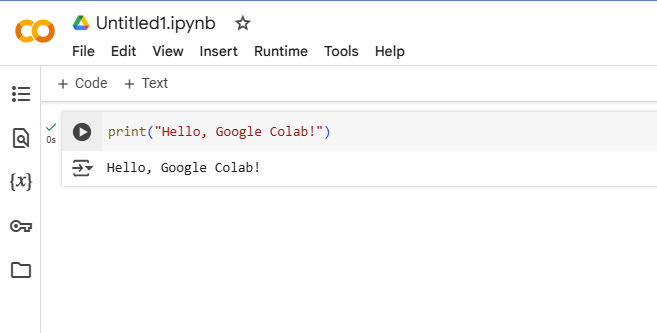
\includegraphics{../images/im222.png}
\end{frame}

\begin{frame}[fragile]{Installing Packages}
\phantomsection\label{installing-packages}
\AddToHookNext{env/Highlighting/begin}{\tiny}

\begin{Shaded}
\begin{Highlighting}[]
\OperatorTok{!}\NormalTok{pip install numpy pandas matplotlib}
\end{Highlighting}
\end{Shaded}

\begin{itemize}
\tightlist
\item
  Use \texttt{!pip\ install} to install Python packages.
\item
  \textbf{Colab comes with pre-installed packages} like NumPy, Pandas,
  Matplotlib, and TensorFlow.
\end{itemize}
\end{frame}

\begin{frame}[fragile]{Using Google Drive with Colab}
\phantomsection\label{using-google-drive-with-colab}
\AddToHookNext{env/Highlighting/begin}{\tiny}

\begin{Shaded}
\begin{Highlighting}[]
\ImportTok{from}\NormalTok{ google.colab }\ImportTok{import}\NormalTok{ drive}
\CommentTok{\# Mount Google Drive to access files}
\NormalTok{drive.mount(}\StringTok{\textquotesingle{}/content/drive\textquotesingle{}}\NormalTok{)}
\end{Highlighting}
\end{Shaded}

\begin{itemize}
\tightlist
\item
  This allows you to access files stored in \textbf{Google Drive} from
  Colab.
\end{itemize}
\end{frame}

\begin{frame}[fragile]{Uploading and Downloading Files}
\phantomsection\label{uploading-and-downloading-files}
\AddToHookNext{env/Highlighting/begin}{\tiny}

\begin{Shaded}
\begin{Highlighting}[]
\ImportTok{from}\NormalTok{ google.colab }\ImportTok{import}\NormalTok{ files}

\CommentTok{\# Upload a file}
\NormalTok{uploaded }\OperatorTok{=}\NormalTok{ files.upload()}

\CommentTok{\# Download a file}
\NormalTok{files.download(}\StringTok{"example.csv"}\NormalTok{)}
\end{Highlighting}
\end{Shaded}
\end{frame}

\begin{frame}[fragile]{Creating and Plotting Data with Matplotlib}
\phantomsection\label{creating-and-plotting-data-with-matplotlib}
\AddToHookNext{env/Highlighting/begin}{\tiny}

\begin{Shaded}
\begin{Highlighting}[]
\ImportTok{import}\NormalTok{ numpy }\ImportTok{as}\NormalTok{ np}
\ImportTok{import}\NormalTok{ matplotlib.pyplot }\ImportTok{as}\NormalTok{ plt}

\NormalTok{x }\OperatorTok{=}\NormalTok{ np.linspace(}\DecValTok{0}\NormalTok{, }\DecValTok{10}\NormalTok{, }\DecValTok{100}\NormalTok{)}
\NormalTok{y }\OperatorTok{=}\NormalTok{ np.sin(x)}

\NormalTok{plt.plot(x, y)}
\NormalTok{plt.title(}\StringTok{"Sine Wave"}\NormalTok{)}
\NormalTok{plt.xlabel(}\StringTok{"X{-}axis"}\NormalTok{)}
\NormalTok{plt.ylabel(}\StringTok{"Y{-}axis"}\NormalTok{)}
\NormalTok{plt.show()}
\end{Highlighting}
\end{Shaded}
\end{frame}

\begin{frame}{Creating and Plotting Data with Matplotlib}
\phantomsection\label{creating-and-plotting-data-with-matplotlib-1}
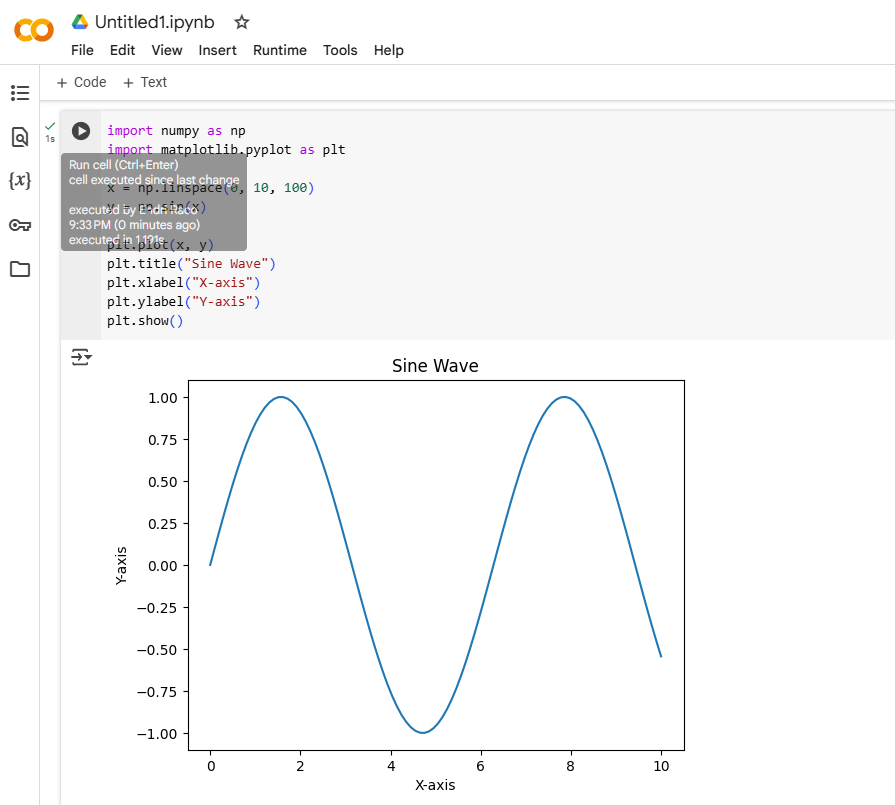
\includegraphics{../images/im223.png}
\end{frame}

\begin{frame}[fragile]{Collaborating in Colab}
\phantomsection\label{collaborating-in-colab}
\begin{itemize}
\item
  Click \textbf{Share} (top right) to invite collaborators.
\item
  Multiple users can edit the same notebook in real-time.
\item
  Version history is automatically saved. \#\# Exporting Notebooks
\item
  Save notebooks in \textbf{Google Drive}.
\item
  Download as \textbf{.ipynb} or \textbf{.py}
  (\texttt{File\ →\ Download}).
\item
  Convert to \textbf{HTML, PDF, or Markdown} using:
\end{itemize}

\begin{Shaded}
\begin{Highlighting}[]
\OperatorTok{!}\NormalTok{jupyter nbconvert }\OperatorTok{{-}{-}}\NormalTok{to html notebook.ipynb}
\end{Highlighting}
\end{Shaded}
\end{frame}

\begin{frame}{Let's get started}
\phantomsection\label{lets-get-started}
\begin{itemize}
\tightlist
\item
  Import the \textbf{matplotlib.pyplot} API, using the conventional name
  plt.
\item
  Create Figure and Axes objects using the \textbf{plt.subplots}
  function.
\item
  Show the results, an empty set of axes, using the plt.show function.
\end{itemize}
\end{frame}

\begin{frame}[fragile]{Let's get started}
\phantomsection\label{lets-get-started-1}
\begin{Shaded}
\begin{Highlighting}[]
\CommentTok{\# Import the matplotlib.pyplot submodule and name it plt}
\ImportTok{import}\NormalTok{ matplotlib.pyplot }\ImportTok{as}\NormalTok{ plt}

\CommentTok{\# Create a Figure and an Axes with plt.subplots}
\NormalTok{fig, ax }\OperatorTok{=}\NormalTok{ plt.subplots()}

\CommentTok{\# Call the show function to show the result}
\NormalTok{plt.show()}
\end{Highlighting}
\end{Shaded}
\end{frame}

\begin{frame}{Let's get started}
\phantomsection\label{lets-get-started-2}
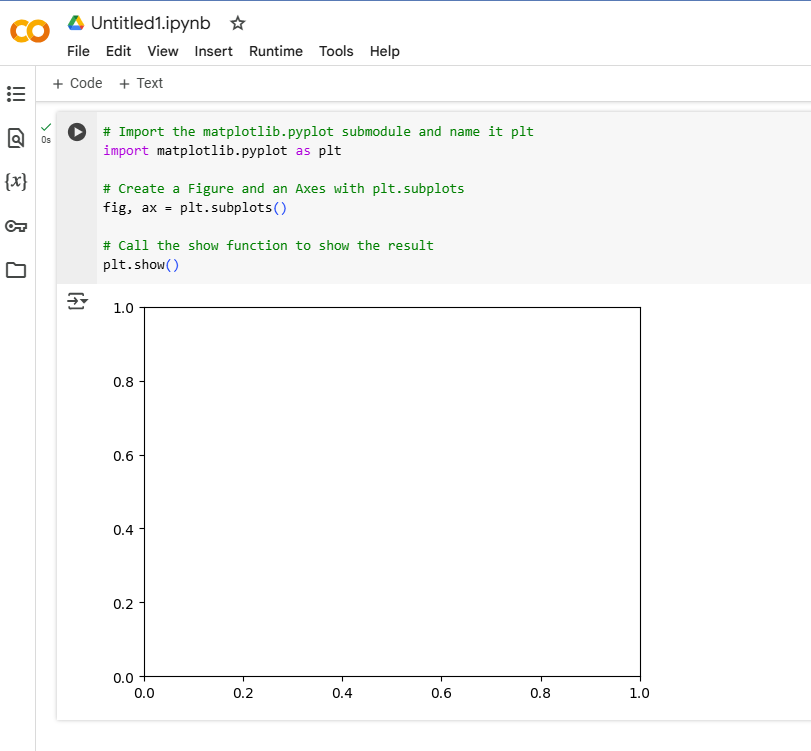
\includegraphics{../images/im224}
\end{frame}

\begin{frame}{Adding data to an Axes object}
\phantomsection\label{adding-data-to-an-axes-object}
\begin{itemize}
\tightlist
\item
  Adding data to a figure is done by calling methods of the
  \textbf{Axes} object.
\item
  In this exercise, we will use the plot method to add data about
  rainfall in two American cities: Seattle, WA and Austin, TX.
\end{itemize}
\end{frame}

\begin{frame}[fragile]{Adding data to an Axes object}
\phantomsection\label{adding-data-to-an-axes-object-1}
seattle\_weather stores information about the weather in Seattle, and
austin\_weather stores information about the weather in Austin.

\AddToHookNext{env/Highlighting/begin}{\tiny}

\begin{Shaded}
\begin{Highlighting}[]
\ImportTok{import}\NormalTok{ pandas }\ImportTok{as}\NormalTok{ pd}

\CommentTok{\# URLs for the datasets}
\NormalTok{seattle\_url }\OperatorTok{=} \StringTok{"https://raw.githubusercontent.com/endri81/DataVisualization/refs/heads/main/data/seattle\_weather.csv"}
\NormalTok{austin\_url }\OperatorTok{=} \StringTok{"https://raw.githubusercontent.com/endri81/DataVisualization/refs/heads/main/data/austin\_weather.csv"}

\CommentTok{\# Load datasets}
\NormalTok{seattle\_weather }\OperatorTok{=}\NormalTok{ pd.read\_csv(seattle\_url)}
\NormalTok{austin\_weather }\OperatorTok{=}\NormalTok{ pd.read\_csv(austin\_url)}
\end{Highlighting}
\end{Shaded}
\end{frame}

\begin{frame}[fragile]{Adding data to an Axes object}
\phantomsection\label{adding-data-to-an-axes-object-2}
\AddToHookNext{env/Highlighting/begin}{\tiny}

\begin{Shaded}
\begin{Highlighting}[]
\CommentTok{\# Display first few rows}
\BuiltInTok{print}\NormalTok{(}\StringTok{"Seattle Weather:"}\NormalTok{)}
\BuiltInTok{print}\NormalTok{(seattle\_weather.head())}
\BuiltInTok{print}\NormalTok{(}\StringTok{"}\CharTok{\textbackslash{}n}\StringTok{Austin Weather:"}\NormalTok{)}
\BuiltInTok{print}\NormalTok{(austin\_weather.head())}
\end{Highlighting}
\end{Shaded}
\end{frame}

\begin{frame}{Adding data to an Axes object}
\phantomsection\label{adding-data-to-an-axes-object-3}
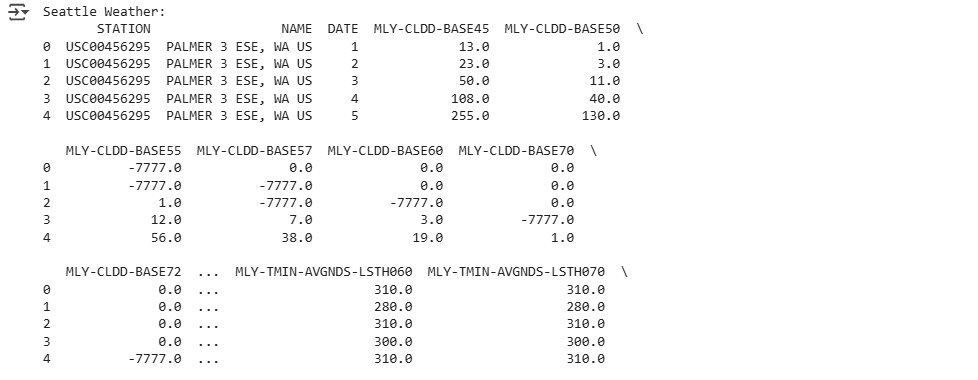
\includegraphics{../images/im225.png}
\end{frame}

\begin{frame}[fragile]{Adding data to an Axes object}
\phantomsection\label{adding-data-to-an-axes-object-4}
\AddToHookNext{env/Highlighting/begin}{\tiny}

\begin{Shaded}
\begin{Highlighting}[]
\NormalTok{austin\_weather[}\StringTok{"MONTH"}\NormalTok{] }\OperatorTok{=}\NormalTok{ austin\_weather[}\StringTok{"DATE"}\NormalTok{]}
\NormalTok{seattle\_weather }\OperatorTok{=}\NormalTok{ seattle\_weather[seattle\_weather[}\StringTok{"STATION"}\NormalTok{] }\OperatorTok{==} \StringTok{"USW00094290"}\NormalTok{]}
\NormalTok{seattle\_weather[}\StringTok{"MONTH"}\NormalTok{] }\OperatorTok{=}\NormalTok{ seattle\_weather[}\StringTok{"DATE"}\NormalTok{]}
\end{Highlighting}
\end{Shaded}
\end{frame}

\section{Creating Basic Plots}\label{creating-basic-plots}

\begin{frame}{The Pyplot Interface}
\phantomsection\label{the-pyplot-interface}
Matplotlib's pyplot module allows quick creation of plots. The basic
structure involves:

\begin{itemize}
\tightlist
\item
  Creating a Figure and Axes.
\item
  Adding data to the Axes.
\item
  Displaying the plot.
\end{itemize}
\end{frame}

\begin{frame}[fragile]{The Pyplot Interface}
\phantomsection\label{the-pyplot-interface-1}
\begin{Shaded}
\begin{Highlighting}[]
\ImportTok{import}\NormalTok{ matplotlib.pyplot }\ImportTok{as}\NormalTok{ plt}
\NormalTok{fig, ax }\OperatorTok{=}\NormalTok{ plt.subplots()}
\CommentTok{\# Adding data to the plot}
\NormalTok{ax.plot(seattle\_weather[}\StringTok{"MONTH"}\NormalTok{], seattle\_weather[}\StringTok{"MLY{-}TAVG{-}NORMAL"}\NormalTok{])}
\CommentTok{\# Display the plot}
\NormalTok{plt.show()}
\end{Highlighting}
\end{Shaded}
\end{frame}

\begin{frame}{Adding Data to Plots: Line Plots}
\phantomsection\label{adding-data-to-plots-line-plots}
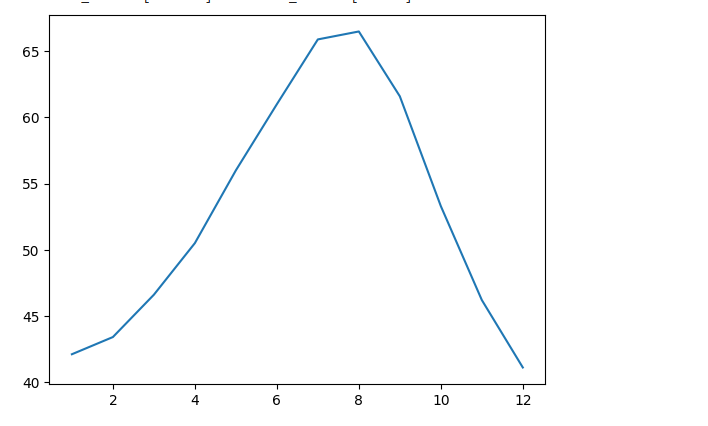
\includegraphics{../images/im226.png}
\end{frame}

\begin{frame}[fragile]{Adding Multiple Lines}
\phantomsection\label{adding-multiple-lines}
We can overlay multiple datasets by calling .plot() multiple times.

\AddToHookNext{env/Highlighting/begin}{\tiny}

\begin{Shaded}
\begin{Highlighting}[]
\ImportTok{import}\NormalTok{ matplotlib.pyplot }\ImportTok{as}\NormalTok{ plt}
\CommentTok{\# Create a blank figure and axes}
\NormalTok{fig, ax }\OperatorTok{=}\NormalTok{ plt.subplots()}
\NormalTok{ax.plot(seattle\_weather[}\StringTok{"MONTH"}\NormalTok{], seattle\_weather[}\StringTok{"MLY{-}TAVG{-}NORMAL"}\NormalTok{], label}\OperatorTok{=}\StringTok{"Seattle"}\NormalTok{)}
\CommentTok{\# Plot Austin data}
\NormalTok{ax.plot(austin\_weather[}\StringTok{"MONTH"}\NormalTok{], austin\_weather[}\StringTok{"MLY{-}TAVG{-}NORMAL"}\NormalTok{], label}\OperatorTok{=}\StringTok{"Austin"}\NormalTok{)}
\CommentTok{\# Add legend}
\NormalTok{ax.legend()}
\NormalTok{plt.show()}
\end{Highlighting}
\end{Shaded}
\end{frame}

\begin{frame}{Adding Multiple Lines}
\phantomsection\label{adding-multiple-lines-1}
\end{frame}

\begin{frame}[fragile]{Customizing Plots:Adding Titles and Labels}
\phantomsection\label{customizing-plotsadding-titles-and-labels}
We can customize our plots by setting labels and titles.

\AddToHookNext{env/Highlighting/begin}{\tiny}

\begin{Shaded}
\begin{Highlighting}[]
\NormalTok{fig, ax }\OperatorTok{=}\NormalTok{ plt.subplots()}
\NormalTok{ax.plot(seattle\_weather[}\StringTok{"MONTH"}\NormalTok{], seattle\_weather[}\StringTok{"MLY{-}TAVG{-}NORMAL"}\NormalTok{])}
\end{Highlighting}
\end{Shaded}
\end{frame}

\begin{frame}{Customizing Plots:Adding Titles and Labels}
\phantomsection\label{customizing-plotsadding-titles-and-labels-1}
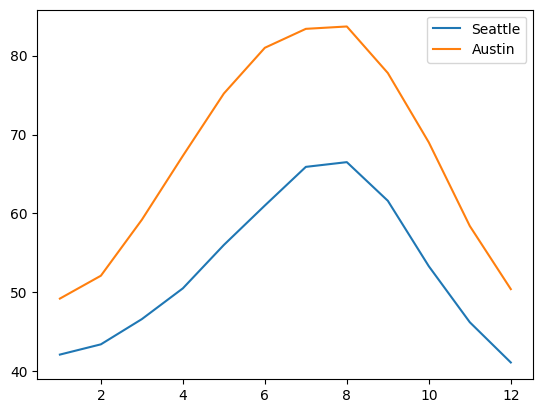
\includegraphics{../images/im227.png}
\end{frame}

\begin{frame}[fragile]{Customizing Plots:Adding Titles and Labels}
\phantomsection\label{customizing-plotsadding-titles-and-labels-2}
\AddToHookNext{env/Highlighting/begin}{\tiny}

\begin{Shaded}
\begin{Highlighting}[]
\ImportTok{import}\NormalTok{ matplotlib.pyplot }\ImportTok{as}\NormalTok{ plt}
\CommentTok{\# Create a blank figure and axes}
\NormalTok{fig, ax }\OperatorTok{=}\NormalTok{ plt.subplots()}
\NormalTok{ax.plot(seattle\_weather[}\StringTok{"MONTH"}\NormalTok{], seattle\_weather[}\StringTok{"MLY{-}TAVG{-}NORMAL"}\NormalTok{], label}\OperatorTok{=}\StringTok{"Seattle"}\NormalTok{)}
\CommentTok{\# Plot Austin data}
\NormalTok{ax.plot(austin\_weather[}\StringTok{"MONTH"}\NormalTok{], austin\_weather[}\StringTok{"MLY{-}TAVG{-}NORMAL"}\NormalTok{], label}\OperatorTok{=}\StringTok{"Austin"}\NormalTok{)}
\CommentTok{\# Add legend}
\NormalTok{ax.legend()}
\CommentTok{\# Adding labels and title}
\NormalTok{ax.set\_xlabel(}\StringTok{"Time (months)"}\NormalTok{)}
\NormalTok{ax.set\_ylabel(}\StringTok{"Average Temperature (°F)"}\NormalTok{)}
\NormalTok{ax.set\_title(}\StringTok{"Seattle Monthly Average Temperature"}\NormalTok{)}
\NormalTok{plt.show()}
\end{Highlighting}
\end{Shaded}
\end{frame}

\begin{frame}{Customizing Plots:Adding Titles and Labels}
\phantomsection\label{customizing-plotsadding-titles-and-labels-3}
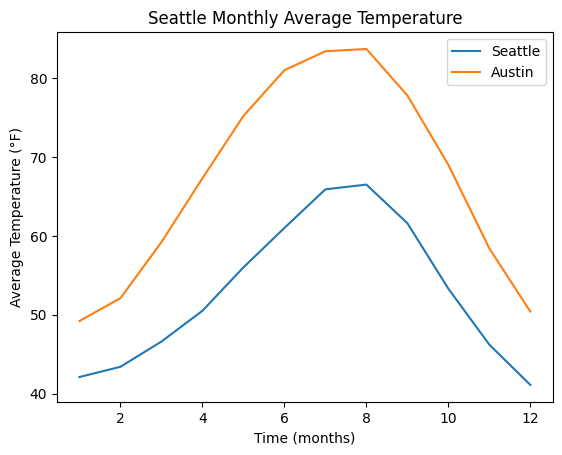
\includegraphics{../images/im228.png}
\end{frame}

\begin{frame}[fragile]{Changing Line Styles and Markers}
\phantomsection\label{changing-line-styles-and-markers}
We can customize line styles (linestyle), colors (color), and markers
(marker).

\AddToHookNext{env/Highlighting/begin}{\tiny}

\begin{Shaded}
\begin{Highlighting}[]
\NormalTok{fig, ax }\OperatorTok{=}\NormalTok{ plt.subplots()}
\NormalTok{ax.plot(seattle\_weather[}\StringTok{"MONTH"}\NormalTok{], seattle\_weather[}\StringTok{"MLY{-}TAVG{-}NORMAL"}\NormalTok{], marker}\OperatorTok{=}\StringTok{"o"}\NormalTok{, linestyle}\OperatorTok{=}\StringTok{"{-}{-}"}\NormalTok{, color}\OperatorTok{=}\StringTok{"r"}\NormalTok{)}
\NormalTok{plt.show()}
\end{Highlighting}
\end{Shaded}
\end{frame}

\begin{frame}{Changing Line Styles and Markers}
\phantomsection\label{changing-line-styles-and-markers-1}
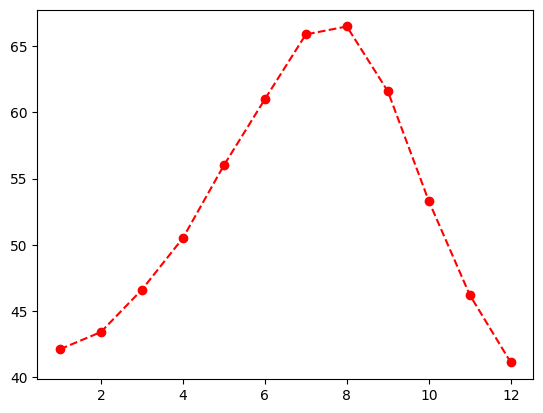
\includegraphics{../images/im230.png}
\end{frame}

\begin{frame}{Changing Line Styles and Markers}
\phantomsection\label{changing-line-styles-and-markers-2}
\begin{itemize}
\tightlist
\item
  marker=``o'' adds circular markers.
\item
  linestyle=``--'' makes a dashed line.
\item
  color=``r'' makes the line red.
\end{itemize}
\end{frame}

\begin{frame}[fragile]{Using Subplots: Creating Multiple Subplots}
\phantomsection\label{using-subplots-creating-multiple-subplots}
We can create multiple smaller plots within a single figure.

\AddToHookNext{env/Highlighting/begin}{\tiny}

\begin{Shaded}
\begin{Highlighting}[]
\CommentTok{\# Create a Figure and an array of subplots with 2 rows and 2 columns}
\NormalTok{fig, ax }\OperatorTok{=}\NormalTok{ plt.subplots(}\DecValTok{2}\NormalTok{, }\DecValTok{2}\NormalTok{)}

\CommentTok{\# Addressing the top left Axes as index 0, 0, plot month and Seattle precipitation}
\NormalTok{ax[}\DecValTok{0}\NormalTok{, }\DecValTok{0}\NormalTok{].plot(seattle\_weather[}\StringTok{"MONTH"}\NormalTok{], seattle\_weather[}\StringTok{"MLY{-}PRCP{-}NORMAL"}\NormalTok{])}

\CommentTok{\# In the top right (index 0,1), plot month and Seattle temperatures}
\NormalTok{ax[}\DecValTok{0}\NormalTok{, }\DecValTok{1}\NormalTok{].plot(seattle\_weather[}\StringTok{"MONTH"}\NormalTok{], seattle\_weather[}\StringTok{"MLY{-}TAVG{-}NORMAL"}\NormalTok{])}

\CommentTok{\# In the bottom left (1, 0) plot month and Austin precipitations}
\NormalTok{ax[}\DecValTok{1}\NormalTok{, }\DecValTok{0}\NormalTok{].plot(austin\_weather[}\StringTok{"MONTH"}\NormalTok{], austin\_weather[}\StringTok{"MLY{-}PRCP{-}NORMAL"}\NormalTok{])}

\CommentTok{\# In the bottom right (1, 1) plot month and Austin temperatures}
\NormalTok{ax[}\DecValTok{1}\NormalTok{, }\DecValTok{1}\NormalTok{].plot(austin\_weather[}\StringTok{"MONTH"}\NormalTok{], austin\_weather[}\StringTok{"MLY{-}TAVG{-}NORMAL"}\NormalTok{])}
\NormalTok{plt.show()}
\end{Highlighting}
\end{Shaded}
\end{frame}

\begin{frame}{Using Subplots: Creating Multiple Subplots}
\phantomsection\label{using-subplots-creating-multiple-subplots-1}
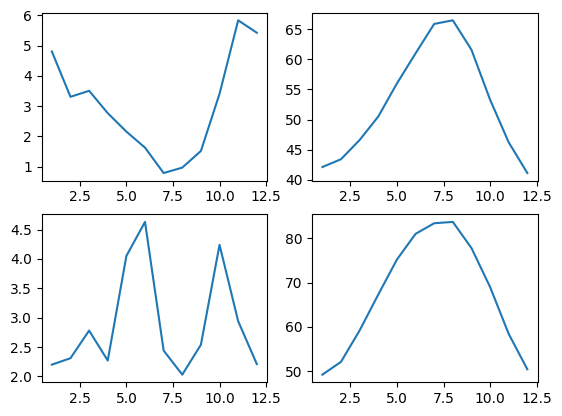
\includegraphics{../images/im231.png}
\end{frame}

\begin{frame}{Small multiples with shared y axis}
\phantomsection\label{small-multiples-with-shared-y-axis}
When creating small multiples, it is often preferable to make sure that
the different plots are displayed with the same scale used on the
y-axis.

This can be configured by setting the sharey key-word to True.
\end{frame}

\begin{frame}{Small multiples with shared y axis}
\phantomsection\label{small-multiples-with-shared-y-axis-1}
In this exercise, you will create a Figure with two Axes objects that
share their y-axis.

As before, the data is provided in seattle\_weather and austin\_weather
DataFrames.
\end{frame}

\begin{frame}[fragile]{Small multiples with shared y axis}
\phantomsection\label{small-multiples-with-shared-y-axis-2}
\AddToHookNext{env/Highlighting/begin}{\tiny}

\begin{Shaded}
\begin{Highlighting}[]
\CommentTok{\# Create a figure and an array of axes: 2 rows, 1 column with shared y axis}
\NormalTok{fig, ax }\OperatorTok{=}\NormalTok{ plt.subplots(}\DecValTok{2}\NormalTok{, }\DecValTok{1}\NormalTok{, sharey}\OperatorTok{=}\VariableTok{True}\NormalTok{)}

\CommentTok{\# Plot Seattle precipitation in the top axes}
\NormalTok{ax[}\DecValTok{0}\NormalTok{].plot(seattle\_weather[}\StringTok{"MONTH"}\NormalTok{], seattle\_weather[}\StringTok{"MLY{-}PRCP{-}NORMAL"}\NormalTok{], color}\OperatorTok{=}\StringTok{\textquotesingle{}b\textquotesingle{}}\NormalTok{)}
\NormalTok{ax[}\DecValTok{0}\NormalTok{].plot(seattle\_weather[}\StringTok{"MONTH"}\NormalTok{], seattle\_weather[}\StringTok{"MLY{-}PRCP{-}25PCTL"}\NormalTok{], color}\OperatorTok{=}\StringTok{\textquotesingle{}b\textquotesingle{}}\NormalTok{, linestyle}\OperatorTok{=}\StringTok{\textquotesingle{}{-}{-}\textquotesingle{}}\NormalTok{)}
\NormalTok{ax[}\DecValTok{0}\NormalTok{].plot(seattle\_weather[}\StringTok{"MONTH"}\NormalTok{], seattle\_weather[}\StringTok{"MLY{-}PRCP{-}75PCTL"}\NormalTok{], color}\OperatorTok{=}\StringTok{\textquotesingle{}b\textquotesingle{}}\NormalTok{, linestyle}\OperatorTok{=}\StringTok{\textquotesingle{}{-}{-}\textquotesingle{}}\NormalTok{)}
\end{Highlighting}
\end{Shaded}
\end{frame}

\begin{frame}[fragile]{Small multiples with shared y axis}
\phantomsection\label{small-multiples-with-shared-y-axis-3}
\AddToHookNext{env/Highlighting/begin}{\tiny}

\begin{Shaded}
\begin{Highlighting}[]
\CommentTok{\# Plot Austin precipitation in the bottom axes}
\NormalTok{ax[}\DecValTok{1}\NormalTok{].plot(austin\_weather[}\StringTok{"MONTH"}\NormalTok{], austin\_weather[}\StringTok{"MLY{-}PRCP{-}NORMAL"}\NormalTok{], color}\OperatorTok{=}\StringTok{\textquotesingle{}r\textquotesingle{}}\NormalTok{)}
\NormalTok{ax[}\DecValTok{1}\NormalTok{].plot(austin\_weather[}\StringTok{"MONTH"}\NormalTok{], austin\_weather[}\StringTok{"MLY{-}PRCP{-}25PCTL"}\NormalTok{], color}\OperatorTok{=}\StringTok{\textquotesingle{}r\textquotesingle{}}\NormalTok{, linestyle}\OperatorTok{=}\StringTok{\textquotesingle{}{-}{-}\textquotesingle{}}\NormalTok{)}
\NormalTok{ax[}\DecValTok{1}\NormalTok{].plot(austin\_weather[}\StringTok{"MONTH"}\NormalTok{], austin\_weather[}\StringTok{"MLY{-}PRCP{-}75PCTL"}\NormalTok{], color}\OperatorTok{=}\StringTok{\textquotesingle{}r\textquotesingle{}}\NormalTok{, linestyle}\OperatorTok{=}\StringTok{\textquotesingle{}{-}{-}\textquotesingle{}}\NormalTok{)}

\NormalTok{plt.show()}
\end{Highlighting}
\end{Shaded}
\end{frame}

\begin{frame}{Small multiples with shared y axis}
\phantomsection\label{small-multiples-with-shared-y-axis-4}
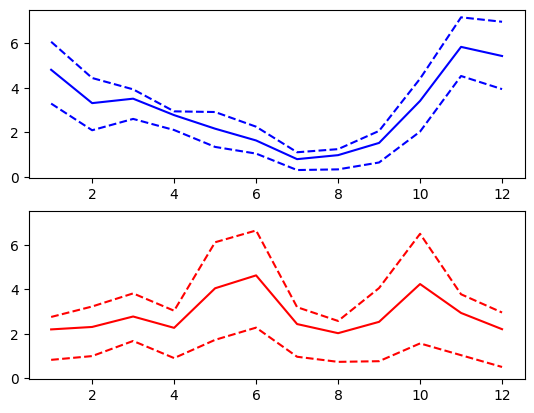
\includegraphics{../images/im232.png}
\end{frame}

\section{Plotting time-series}\label{plotting-time-series}

\begin{frame}{Read data with a time index}
\phantomsection\label{read-data-with-a-time-index}
\textbf{pandas DataFrame} objects can have an index denoting time, this
recognized by Matplotlib for axis labeling.

This exercise involves reading data from climate\_change.csv, containing
CO2 levels and temperatures recorded on the 6th of each month from 1958
to 2016, using pandas' read\_csv function.
\end{frame}

\begin{frame}{Read data with a time index}
\phantomsection\label{read-data-with-a-time-index-1}
The parse\_dates and index\_col arguments help set a DateTimeIndex.

Don't forget to check out the Matplotlib Cheat Sheet for a quick
overview of essential concepts and methods.
\end{frame}

\begin{frame}[fragile]{Read data with a time index}
\phantomsection\label{read-data-with-a-time-index-2}
\AddToHookNext{env/Highlighting/begin}{\tiny}

\begin{Shaded}
\begin{Highlighting}[]
\CommentTok{\# Import pandas}
\ImportTok{import}\NormalTok{ pandas }\ImportTok{as}\NormalTok{ pd}
\end{Highlighting}
\end{Shaded}
\end{frame}

\begin{frame}[fragile]{Read data with a time index}
\phantomsection\label{read-data-with-a-time-index-3}
\AddToHookNext{env/Highlighting/begin}{\tiny}

\begin{Shaded}
\begin{Highlighting}[]
\CommentTok{\# Read the data from file using read\_csv}
\ImportTok{import}\NormalTok{ pandas }\ImportTok{as}\NormalTok{ pd}
\ImportTok{import}\NormalTok{ matplotlib.pyplot }\ImportTok{as}\NormalTok{ plt}
\CommentTok{\# URLs for the datasets}
\NormalTok{climate\_url }\OperatorTok{=} \StringTok{"https://raw.githubusercontent.com/endri81/DataVisualization/refs/heads/main/data/climate\_change.csv"}
\CommentTok{\# Load datasets}
\NormalTok{climate\_change }\OperatorTok{=}\NormalTok{ pd.read\_csv(climate\_url, parse\_dates}\OperatorTok{=}\NormalTok{[}\StringTok{"date"}\NormalTok{], index\_col}\OperatorTok{=}\StringTok{"date"}\NormalTok{)}
\end{Highlighting}
\end{Shaded}
\end{frame}

\begin{frame}{Plot time-series data}
\phantomsection\label{plot-time-series-data}
To plot time-series data, we use the Axes object plot command.

The first argument to this method are the values for the x-axis and the
second argument are the values for the y-axis.
\end{frame}

\begin{frame}{Plot time-series data}
\phantomsection\label{plot-time-series-data-1}
This exercise provides data stored in a DataFrame called
climate\_change.

This variable has a time-index with the dates of measurements and two
data columns: ``co2'' and ``relative\_temp''.
\end{frame}

\begin{frame}{Plot time-series data}
\phantomsection\label{plot-time-series-data-2}
In this case, the index of the DataFrame would be used as the x-axis
values and we will plot the values stored in the ``relative\_temp''
column as the y-axis values.

We will also properly label the x-axis and y-axis.
\end{frame}

\begin{frame}[fragile]{Plot time-series data}
\phantomsection\label{plot-time-series-data-3}
\AddToHookNext{env/Highlighting/begin}{\tiny}

\begin{Shaded}
\begin{Highlighting}[]
\ImportTok{import}\NormalTok{ matplotlib.pyplot }\ImportTok{as}\NormalTok{ plt}
\NormalTok{fig, ax }\OperatorTok{=}\NormalTok{ plt.subplots()}

\CommentTok{\# Add the time{-}series for "relative\_temp" to the plot}
\NormalTok{ax.plot(climate\_change.index, climate\_change[}\StringTok{\textquotesingle{}relative\_temp\textquotesingle{}}\NormalTok{])}
\end{Highlighting}
\end{Shaded}
\end{frame}

\begin{frame}[fragile]{Plot time-series data}
\phantomsection\label{plot-time-series-data-4}
\AddToHookNext{env/Highlighting/begin}{\tiny}

\begin{Shaded}
\begin{Highlighting}[]
\CommentTok{\# Set the x{-}axis label}
\NormalTok{ax.set\_xlabel(}\StringTok{\textquotesingle{}Time\textquotesingle{}}\NormalTok{)}

\CommentTok{\# Set the y{-}axis label }
\NormalTok{ax.set\_ylabel(}\StringTok{\textquotesingle{}Relative temperature (Celsius)\textquotesingle{}}\NormalTok{)}

\CommentTok{\# Show the figure}
\NormalTok{plt.show()}
\end{Highlighting}
\end{Shaded}
\end{frame}

\begin{frame}{Plot time-series data}
\phantomsection\label{plot-time-series-data-5}
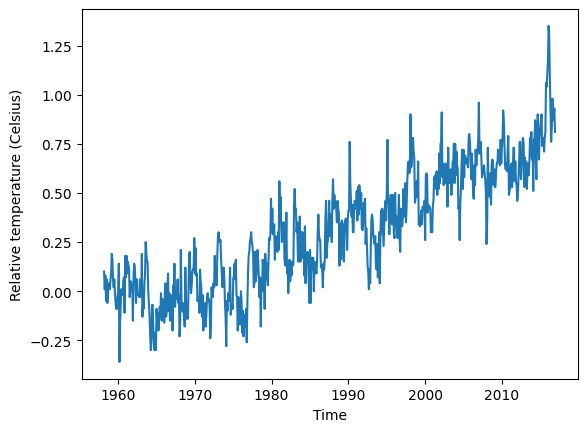
\includegraphics{../images/im233.png}
\end{frame}

\begin{frame}{Using a time index to zoom in}
\phantomsection\label{using-a-time-index-to-zoom-in}
When a time-series is represented with a time index, we can use this
index for the x-axis when plotting.

We can also select a range of dates to zoom in on a particular period
within the time-series using pandas' indexing facilities.
\end{frame}

\begin{frame}{Using a time index to zoom in}
\phantomsection\label{using-a-time-index-to-zoom-in-1}
In this exercise, you will select a portion of a time-series dataset and
you will plot that period.

The data to use is stored in a DataFrame called climate\_change, which
has a time-index with dates of measurements and two data columns:
``co2'' and ``relative\_temp''.
\end{frame}

\begin{frame}[fragile]{Using a time index to zoom in}
\phantomsection\label{using-a-time-index-to-zoom-in-2}
\AddToHookNext{env/Highlighting/begin}{\tiny}

\begin{Shaded}
\begin{Highlighting}[]
\ImportTok{import}\NormalTok{ matplotlib.pyplot }\ImportTok{as}\NormalTok{ plt}

\CommentTok{\# Use plt.subplots to create fig and ax}
\NormalTok{fig, ax }\OperatorTok{=}\NormalTok{ plt.subplots()}

\CommentTok{\# Create variable seventies with data from "1970{-}01{-}01" to "1979{-}12{-}31"}
\NormalTok{seventies }\OperatorTok{=}\NormalTok{ climate\_change[}\StringTok{"1970{-}01{-}01"}\NormalTok{:}\StringTok{"1979{-}12{-}31"}\NormalTok{]}
\end{Highlighting}
\end{Shaded}
\end{frame}

\begin{frame}[fragile]{Using a time index to zoom in}
\phantomsection\label{using-a-time-index-to-zoom-in-3}
\AddToHookNext{env/Highlighting/begin}{\tiny}

\begin{Shaded}
\begin{Highlighting}[]
\CommentTok{\# Add the time{-}series for "co2" data from seventies to the plot}
\NormalTok{ax.plot(seventies.index, seventies[}\StringTok{"co2"}\NormalTok{])}

\CommentTok{\# Show the figure}
\NormalTok{plt.show()}
\end{Highlighting}
\end{Shaded}
\end{frame}

\begin{frame}{Using a time index to zoom in}
\phantomsection\label{using-a-time-index-to-zoom-in-4}
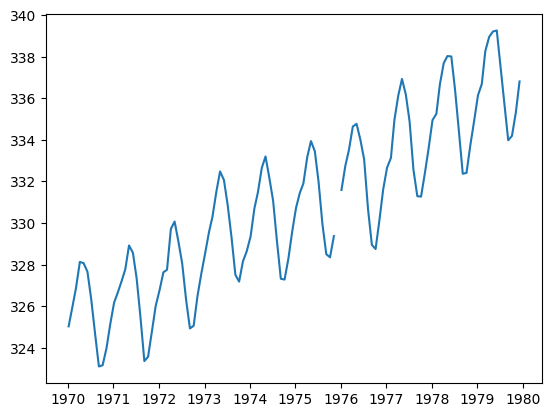
\includegraphics{../images/im234.png}
\end{frame}

\begin{frame}{Plotting two variables}
\phantomsection\label{plotting-two-variables}
If you want to plot two time-series variables that were recorded at the
same times, you can add both of them to the same subplot.

If the variables have very different scales, you'll want to make sure
that you plot them in different twin Axes objects.
\end{frame}

\begin{frame}{Plotting two variables}
\phantomsection\label{plotting-two-variables-1}
These objects can share one axis (for example, the time, or x-axis)
while not sharing the other (the y-axis).

To create a twin Axes object that shares the x-axis, we use the twinx
method.
\end{frame}

\begin{frame}{Plotting two variables}
\phantomsection\label{plotting-two-variables-2}
In this exercise, you'll have access to a DataFrame that has the
climate\_change data loaded into it.

This DataFrame was loaded with the ``date'' column set as a
DateTimeIndex, and it has a column called ``co2'' with carbon dioxide
measurements and a column called ``relative\_temp'' with temperature
measurements.
\end{frame}

\begin{frame}[fragile]{Plotting two variables}
\phantomsection\label{plotting-two-variables-3}
\AddToHookNext{env/Highlighting/begin}{\tiny}

\begin{Shaded}
\begin{Highlighting}[]
\ImportTok{import}\NormalTok{ matplotlib.pyplot }\ImportTok{as}\NormalTok{ plt}

\CommentTok{\# Initalize a Figure and Axes}
\NormalTok{fig, ax }\OperatorTok{=}\NormalTok{ plt.subplots()}

\CommentTok{\# Plot the CO2 variable in blue}
\NormalTok{ax.plot(climate\_change.index, climate\_change[}\StringTok{"co2"}\NormalTok{], color}\OperatorTok{=}\StringTok{\textquotesingle{}blue\textquotesingle{}}\NormalTok{)}
\end{Highlighting}
\end{Shaded}
\end{frame}

\begin{frame}[fragile]{Plotting two variables}
\phantomsection\label{plotting-two-variables-4}
\AddToHookNext{env/Highlighting/begin}{\tiny}

\begin{Shaded}
\begin{Highlighting}[]
\CommentTok{\# Create a twin Axes that shares the x{-}axis}
\NormalTok{ax2 }\OperatorTok{=}\NormalTok{ ax.twinx()}

\CommentTok{\# Plot the relative temperature in red}
\NormalTok{ax2.plot(climate\_change.index, climate\_change[}\StringTok{"relative\_temp"}\NormalTok{], color}\OperatorTok{=}\StringTok{\textquotesingle{}red\textquotesingle{}}\NormalTok{)}

\NormalTok{plt.show()}
\end{Highlighting}
\end{Shaded}
\end{frame}

\begin{frame}{Plotting two variables}
\phantomsection\label{plotting-two-variables-5}
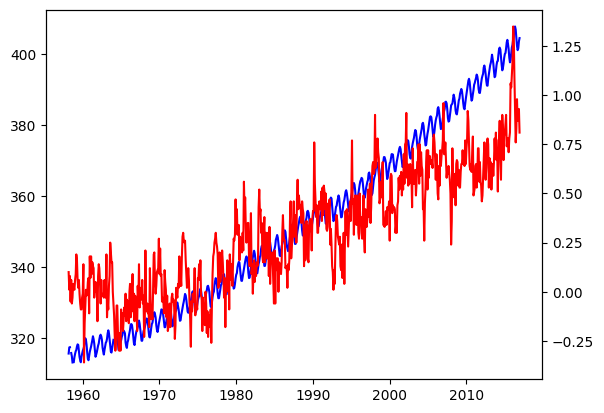
\includegraphics{../images/im235.png}
\end{frame}

\begin{frame}{Defining a function that plots time-series data}
\phantomsection\label{defining-a-function-that-plots-time-series-data}
Once you realize that a particular section of code that you have written
is useful, it is a good idea to define a function that saves that
section of code for you, rather than copying it to other parts of your
program where you would like to use this code.
\end{frame}

\begin{frame}{Defining a function that plots time-series data}
\phantomsection\label{defining-a-function-that-plots-time-series-data-1}
Here, we will define a function that takes inputs such as a time
variable and some other variable and plots them as x and y inputs.

Then, it sets the labels on the x- and y-axis and sets the colors of the
y-axis label, the y-axis ticks and the tick labels.
\end{frame}

\begin{frame}[fragile]{Defining a function that plots time-series data}
\phantomsection\label{defining-a-function-that-plots-time-series-data-2}
\AddToHookNext{env/Highlighting/begin}{\tiny}

\begin{Shaded}
\begin{Highlighting}[]
\CommentTok{\# Define a function called plot\_timeseries}
\KeywordTok{def}\NormalTok{ plot\_timeseries(axes, x, y, color, xlabel, ylabel):}

  \CommentTok{\# Plot the inputs x,y in the provided color}
\NormalTok{  axes.plot(x, y, color}\OperatorTok{=}\NormalTok{color)}

  \CommentTok{\# Set the x{-}axis label}
\NormalTok{  axes.set\_xlabel(xlabel)}
\end{Highlighting}
\end{Shaded}
\end{frame}

\begin{frame}[fragile]{Defining a function that plots time-series data}
\phantomsection\label{defining-a-function-that-plots-time-series-data-3}
\AddToHookNext{env/Highlighting/begin}{\tiny}

\begin{Shaded}
\begin{Highlighting}[]

  \CommentTok{\# Set the y{-}axis label}
\NormalTok{  axes.set\_ylabel(ylabel, color}\OperatorTok{=}\NormalTok{color)}

  \CommentTok{\# Set the colors tick params for y{-}axis}
\NormalTok{  axes.tick\_params(}\StringTok{\textquotesingle{}y\textquotesingle{}}\NormalTok{, colors}\OperatorTok{=}\NormalTok{color)}
\end{Highlighting}
\end{Shaded}
\end{frame}

\begin{frame}{Using a plotting function}
\phantomsection\label{using-a-plotting-function}
Defining functions allows us to reuse the same code without having to
repeat all of it. Programmers sometimes say ``Don't repeat yourself''.
\end{frame}

\begin{frame}[fragile]{Using a plotting function}
\phantomsection\label{using-a-plotting-function-1}
In the previous exercise, you defined a function called
plot\_timeseries:

\AddToHookNext{env/Highlighting/begin}{\tiny}

\begin{Shaded}
\begin{Highlighting}[]
\NormalTok{plot\_timeseries(axes, x, y, color, xlabel, ylabel)}
\end{Highlighting}
\end{Shaded}

that takes an Axes object (as the argument axes), time-series data (as x
and y arguments) the name of a color (as a string, provided as the color
argument) and x-axis and y-axis labels (as xlabel and ylabel arguments).
\end{frame}

\begin{frame}{Using a plotting function}
\phantomsection\label{using-a-plotting-function-2}
In this exercise, the function plot\_timeseries is already defined and
provided to you.

Use this function to plot the climate\_change time-series data, provided
as a pandas DataFrame object that has a DateTimeIndex with the dates of
the measurements and co2 and relative\_temp columns.
\end{frame}

\begin{frame}[fragile]{Using a plotting function}
\phantomsection\label{using-a-plotting-function-3}
\AddToHookNext{env/Highlighting/begin}{\tiny}

\begin{Shaded}
\begin{Highlighting}[]
\NormalTok{fig, ax }\OperatorTok{=}\NormalTok{ plt.subplots()}

\CommentTok{\# Plot the CO2 levels time{-}series in blue}
\NormalTok{plot\_timeseries(ax, climate\_change.index, climate\_change[}\StringTok{"co2"}\NormalTok{], }\StringTok{\textquotesingle{}blue\textquotesingle{}}\NormalTok{, }\StringTok{"Time (years)"}\NormalTok{, }\StringTok{"CO2 levels"}\NormalTok{)}

\CommentTok{\# Create a twin Axes object that shares the x{-}axis}
\NormalTok{ax2 }\OperatorTok{=}\NormalTok{ ax.twinx()}
\end{Highlighting}
\end{Shaded}
\end{frame}

\begin{frame}[fragile]{Using a plotting function}
\phantomsection\label{using-a-plotting-function-4}
\AddToHookNext{env/Highlighting/begin}{\tiny}

\begin{Shaded}
\begin{Highlighting}[]
\CommentTok{\# Plot the relative temperature data in red}
\NormalTok{plot\_timeseries(ax2, climate\_change.index, climate\_change[}\StringTok{\textquotesingle{}relative\_temp\textquotesingle{}}\NormalTok{], }\StringTok{\textquotesingle{}red\textquotesingle{}}\NormalTok{, }\StringTok{"Time (years)"}\NormalTok{, }\StringTok{"Relative temperature (Celsius)"}\NormalTok{)}

\NormalTok{plt.show()}
\end{Highlighting}
\end{Shaded}
\end{frame}

\begin{frame}{Using a plotting function}
\phantomsection\label{using-a-plotting-function-5}
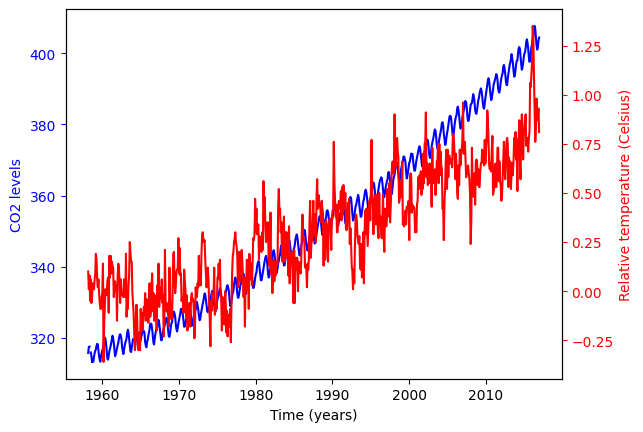
\includegraphics{../images/im236.png}
\end{frame}

\begin{frame}{Annotating a plot of time-series data}
\phantomsection\label{annotating-a-plot-of-time-series-data}
Annotating a plot allows us to highlight interesting information in the
plot.

For example, in describing the climate change dataset, we might want to
point to the date at which the relative temperature first exceeded 1
degree Celsius.
\end{frame}

\begin{frame}{Annotating a plot of time-series data}
\phantomsection\label{annotating-a-plot-of-time-series-data-1}
For this, we will use the annotate method of the Axes object.

In this exercise, you will have the DataFrame called climate\_change
loaded into memory.

Using the Axes methods, plot only the relative temperature column as a
function of dates, and annotate the data.
\end{frame}

\begin{frame}[fragile]{Annotating a plot of time-series data}
\phantomsection\label{annotating-a-plot-of-time-series-data-2}
\AddToHookNext{env/Highlighting/begin}{\tiny}

\begin{Shaded}
\begin{Highlighting}[]
\NormalTok{fig, ax }\OperatorTok{=}\NormalTok{ plt.subplots()}

\CommentTok{\# Plot the relative temperature data}
\NormalTok{ax.plot(climate\_change.index, climate\_change[}\StringTok{\textquotesingle{}relative\_temp\textquotesingle{}}\NormalTok{])}

\CommentTok{\# Annotate the date at which temperatures exceeded 1 degree}
\NormalTok{ax.annotate(}\StringTok{"\textgreater{}1 degree"}\NormalTok{, xy}\OperatorTok{=}\NormalTok{(pd.Timestamp(}\StringTok{\textquotesingle{}2015{-}10{-}06\textquotesingle{}}\NormalTok{), }\DecValTok{1}\NormalTok{))}

\NormalTok{plt.show()}
\end{Highlighting}
\end{Shaded}
\end{frame}

\begin{frame}{Annotating a plot of time-series data}
\phantomsection\label{annotating-a-plot-of-time-series-data-3}
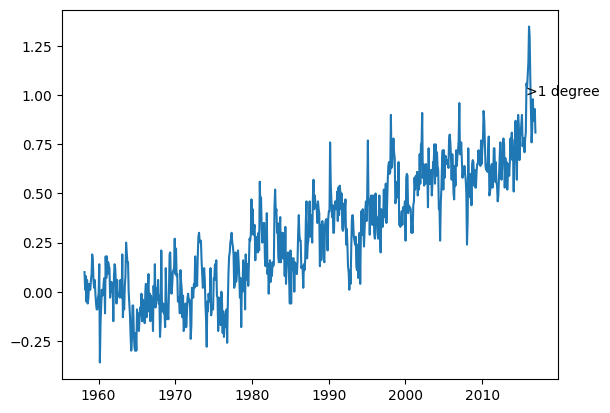
\includegraphics{../images/im237.png}
\end{frame}

\begin{frame}{Plotting time-series: putting it all together}
\phantomsection\label{plotting-time-series-putting-it-all-together}
In this exercise, you will plot two time-series with different scales on
the same Axes, and annotate the data from one of these series.

The CO2/temperatures data is provided as a DataFrame called
climate\_change.
\end{frame}

\begin{frame}{Plotting time-series: putting it all together}
\phantomsection\label{plotting-time-series-putting-it-all-together-1}
You should also use the function that we have defined before, called
plot\_timeseries, which takes an Axes object (as the axes argument)
plots a time-series (provided as x and y arguments), sets the labels for
the x-axis and y-axis and sets the color for the data, and for the y
tick/axis labels:
\end{frame}

\begin{frame}[fragile]{Plotting time-series: putting it all together}
\phantomsection\label{plotting-time-series-putting-it-all-together-2}
\AddToHookNext{env/Highlighting/begin}{\tiny}

\begin{Shaded}
\begin{Highlighting}[]
\NormalTok{plot\_timeseries(axes, x, y, color, xlabel, ylabel)}
\end{Highlighting}
\end{Shaded}
\end{frame}

\begin{frame}{Plotting time-series: putting it all together}
\phantomsection\label{plotting-time-series-putting-it-all-together-3}
Then, you will annotate with text an important time-point in the data:
on 2015-10-06, when the temperature first rose to above 1 degree over
the average.
\end{frame}

\begin{frame}[fragile]{Plotting time-series: putting it all together}
\phantomsection\label{plotting-time-series-putting-it-all-together-4}
\AddToHookNext{env/Highlighting/begin}{\tiny}

\begin{Shaded}
\begin{Highlighting}[]

\NormalTok{fig, ax }\OperatorTok{=}\NormalTok{ plt.subplots()}

\CommentTok{\# Plot the CO2 levels time{-}series in blue}
\NormalTok{plot\_timeseries(ax, climate\_change.index, climate\_change[}\StringTok{"co2"}\NormalTok{], }\StringTok{\textquotesingle{}blue\textquotesingle{}}\NormalTok{, }\StringTok{"Time (years)"}\NormalTok{, }\StringTok{"CO2 levels"}\NormalTok{)}

\CommentTok{\# Create an Axes object that shares the x{-}axis}
\NormalTok{ax2 }\OperatorTok{=}\NormalTok{ ax.twinx()}
\end{Highlighting}
\end{Shaded}
\end{frame}

\begin{frame}[fragile]{Plotting time-series: putting it all together}
\phantomsection\label{plotting-time-series-putting-it-all-together-5}
\AddToHookNext{env/Highlighting/begin}{\tiny}

\begin{Shaded}
\begin{Highlighting}[]

\CommentTok{\# Plot the relative temperature data in red}
\NormalTok{plot\_timeseries(ax2, climate\_change.index, climate\_change[}\StringTok{\textquotesingle{}relative\_temp\textquotesingle{}}\NormalTok{], }\StringTok{\textquotesingle{}red\textquotesingle{}}\NormalTok{, }\StringTok{"Time (years)"}\NormalTok{, }\StringTok{"Relative temp (Celsius)"}\NormalTok{)}

\CommentTok{\# Annotate the point with relative temperature \textgreater{}1 degree}
\NormalTok{ax2.annotate(}\StringTok{"\textgreater{}1 degree"}\NormalTok{, xy}\OperatorTok{=}\NormalTok{(pd.Timestamp(}\StringTok{\textquotesingle{}2015{-}10{-}06\textquotesingle{}}\NormalTok{), }\DecValTok{1}\NormalTok{), xytext}\OperatorTok{=}\NormalTok{(pd.Timestamp(}\StringTok{\textquotesingle{}2008{-}10{-}06\textquotesingle{}}\NormalTok{), }\OperatorTok{{-}}\FloatTok{0.2}\NormalTok{), arrowprops}\OperatorTok{=}\NormalTok{\{}\StringTok{\textquotesingle{}arrowstyle\textquotesingle{}}\NormalTok{:}\StringTok{\textquotesingle{}{-}\textgreater{}\textquotesingle{}}\NormalTok{, }\StringTok{\textquotesingle{}color\textquotesingle{}}\NormalTok{:}\StringTok{\textquotesingle{}gray\textquotesingle{}}\NormalTok{\})}

\NormalTok{plt.show()}
\end{Highlighting}
\end{Shaded}
\end{frame}

\begin{frame}{Plotting time-series: putting it all together}
\phantomsection\label{plotting-time-series-putting-it-all-together-6}
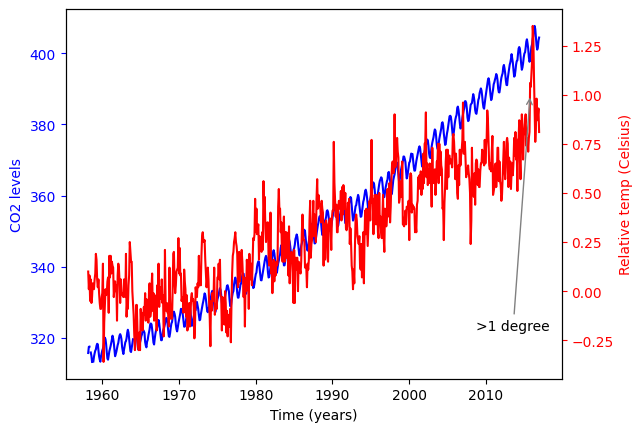
\includegraphics{../images/im239.png}
\end{frame}

\section{Quantitative comparisons and statistical
visualizations}\label{quantitative-comparisons-and-statistical-visualizations}

\begin{frame}{Bar chart}
\phantomsection\label{bar-chart}
Bar charts visualize data that is organized according to categories as a
series of bars, where the height of each bar represents the values of
the data in this category.
\end{frame}

\begin{frame}{Bar chart}
\phantomsection\label{bar-chart-1}
For example, in this exercise, you will visualize the number of gold
medals won by each country in the provided medals DataFrame.

The DataFrame contains the countries as the index, and a column called
``Gold'' that contains the number of gold medals won by each country,
according to their rows.
\end{frame}

\begin{frame}[fragile]{Bar chart}
\phantomsection\label{bar-chart-2}
\AddToHookNext{env/Highlighting/begin}{\tiny}

\begin{Shaded}
\begin{Highlighting}[]
\ImportTok{import}\NormalTok{ pandas }\ImportTok{as}\NormalTok{ pd}
\ImportTok{import}\NormalTok{ matplotlib.pyplot }\ImportTok{as}\NormalTok{ plt}

\CommentTok{\# URL for the dataset}
\NormalTok{medals\_url }\OperatorTok{=} \StringTok{"https://raw.githubusercontent.com/endri81/DataVisualization/refs/heads/main/data/medals\_by\_country\_2016.csv"}

\CommentTok{\# Load dataset}
\NormalTok{medals }\OperatorTok{=}\NormalTok{ pd.read\_csv(medals\_url)}

\CommentTok{\# Set \textquotesingle{}Country\textquotesingle{} as index if it\textquotesingle{}s not already}
\ControlFlowTok{if} \StringTok{"Country"} \KeywordTok{in}\NormalTok{ medals.columns:}
\NormalTok{    medals.set\_index(}\StringTok{"Country"}\NormalTok{, inplace}\OperatorTok{=}\VariableTok{True}\NormalTok{)}


\end{Highlighting}
\end{Shaded}
\end{frame}

\begin{frame}[fragile]{Bar chart}
\phantomsection\label{bar-chart-3}
\AddToHookNext{env/Highlighting/begin}{\tiny}

\begin{Shaded}
\begin{Highlighting}[]
\CommentTok{\# Create figure and axis}
\NormalTok{fig, ax }\OperatorTok{=}\NormalTok{ plt.subplots()}

\CommentTok{\# Plot a bar chart of gold medals as a function of country}
\NormalTok{ax.bar(medals.index, medals[}\StringTok{"Gold"}\NormalTok{])}

\CommentTok{\# Set the x{-}axis tick labels to the country names}
\NormalTok{ax.set\_xticks(}\BuiltInTok{range}\NormalTok{(}\BuiltInTok{len}\NormalTok{(medals.index)))  }\CommentTok{\# Set tick positions}
\NormalTok{ax.set\_xticklabels(medals.index, rotation}\OperatorTok{=}\DecValTok{90}\NormalTok{)  }\CommentTok{\# Set tick labels}

\CommentTok{\# Set the y{-}axis label}
\NormalTok{ax.set\_ylabel(}\StringTok{"Number of Gold Medals"}\NormalTok{)}

\CommentTok{\# Display the plot}
\NormalTok{plt.show()}
\end{Highlighting}
\end{Shaded}
\end{frame}

\begin{frame}{Bar chart}
\phantomsection\label{bar-chart-4}
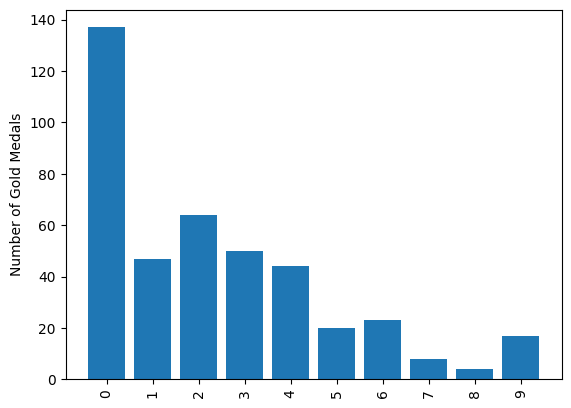
\includegraphics{../images/im240.png}
\end{frame}

\begin{frame}{Stacked bar chart}
\phantomsection\label{stacked-bar-chart}
A stacked bar chart contains bars, where the height of each bar
represents values.

In addition, stacked on top of the first variable may be another
variable.
\end{frame}

\begin{frame}{Stacked bar chart}
\phantomsection\label{stacked-bar-chart-1}
The additional height of this bar represents the value of this variable.
And you can add more bars on top of that.

In this exercise, you will have access to a DataFrame called medals that
contains an index that holds the names of different countries, and three
columns: ``Gold'', ``Silver'' and ``Bronze''.
\end{frame}

\begin{frame}{Stacked bar chart}
\phantomsection\label{stacked-bar-chart-2}
You will also have a Figure, fig, and Axes, ax, that you can add data
to.

You will create a stacked bar chart that shows the number of gold,
silver, and bronze medals won by each country, and you will add labels
and create a legend that indicates which bars represent which medals.
\end{frame}

\begin{frame}[fragile]{Stacked bar chart}
\phantomsection\label{stacked-bar-chart-3}
\AddToHookNext{env/Highlighting/begin}{\tiny}

\begin{Shaded}
\begin{Highlighting}[]
\NormalTok{fig, ax }\OperatorTok{=}\NormalTok{ plt.subplots()}

\CommentTok{\# Add bars for "Gold" with the label "Gold"}
\NormalTok{ax.bar(medals.index, medals[}\StringTok{"Gold"}\NormalTok{], label}\OperatorTok{=}\StringTok{"Gold"}\NormalTok{)}

\CommentTok{\# Stack bars for "Silver" on top with label "Silver"}
\NormalTok{ax.bar(medals.index, medals[}\StringTok{"Silver"}\NormalTok{], bottom}\OperatorTok{=}\NormalTok{medals[}\StringTok{"Gold"}\NormalTok{], label}\OperatorTok{=}\StringTok{"Silver"}\NormalTok{)}
\end{Highlighting}
\end{Shaded}
\end{frame}

\begin{frame}[fragile]{Stacked bar chart}
\phantomsection\label{stacked-bar-chart-4}
\AddToHookNext{env/Highlighting/begin}{\tiny}

\begin{Shaded}
\begin{Highlighting}[]
\CommentTok{\# Stack bars for "Bronze" on top of that with label "Bronze"}
\NormalTok{ax.bar(medals.index, medals[}\StringTok{"Bronze"}\NormalTok{], bottom}\OperatorTok{=}\NormalTok{medals[}\StringTok{"Gold"}\NormalTok{] }\OperatorTok{+}\NormalTok{ medals[}\StringTok{"Silver"}\NormalTok{], label}\OperatorTok{=}\StringTok{"Bronze"}\NormalTok{)}

\CommentTok{\# Display the legend}
\NormalTok{ax.legend()}

\NormalTok{plt.show()}
\end{Highlighting}
\end{Shaded}
\end{frame}

\begin{frame}{Stacked bar chart}
\phantomsection\label{stacked-bar-chart-5}
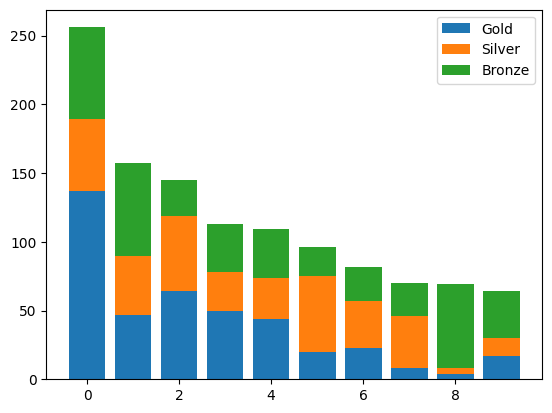
\includegraphics{../images/im241.png}
\end{frame}

\begin{frame}{Creating histograms}
\phantomsection\label{creating-histograms}
Histograms show the full distribution of a variable.

In this exercise, we will display the distribution of weights of
medalists in gymnastics and in rowing in the 2016 Olympic games for a
comparison between them.
\end{frame}

\begin{frame}{Creating histograms}
\phantomsection\label{creating-histograms-1}
You will have two DataFrames to use.

The first is called mens\_rowing and includes information about the
medalists in the men's rowing events.

The other is called mens\_gymnastics and includes information about
medalists in all of the Gymnastics events.
\end{frame}

\begin{frame}[fragile]{Creating histograms}
\phantomsection\label{creating-histograms-2}
\AddToHookNext{env/Highlighting/begin}{\tiny}

\begin{Shaded}
\begin{Highlighting}[]
\ImportTok{import}\NormalTok{ pandas }\ImportTok{as}\NormalTok{ pd}
\ImportTok{import}\NormalTok{ matplotlib.pyplot }\ImportTok{as}\NormalTok{ plt}

\CommentTok{\# URL for the dataset}
\NormalTok{summer\_medals\_url }\OperatorTok{=} \StringTok{"https://raw.githubusercontent.com/endri81/DataVisualization/refs/heads/main/data/summer2016.csv"}

\CommentTok{\# Load dataset}
\NormalTok{summer\_2016\_medals }\OperatorTok{=}\NormalTok{ pd.read\_csv(summer\_medals\_url)}

\CommentTok{\# Set \textquotesingle{}Country\textquotesingle{} as index if it\textquotesingle{}s not already}
\ControlFlowTok{if} \StringTok{"Country"} \KeywordTok{in}\NormalTok{ medals.columns:}
\NormalTok{    medals.set\_index(}\StringTok{"Country"}\NormalTok{, inplace}\OperatorTok{=}\VariableTok{True}\NormalTok{)}
\end{Highlighting}
\end{Shaded}

\AddToHookNext{env/Highlighting/begin}{\tiny}

\begin{Shaded}
\begin{Highlighting}[]
\NormalTok{mens\_rowing }\OperatorTok{=}\NormalTok{ summer\_2016\_medals[(summer\_2016\_medals[}\StringTok{\textquotesingle{}Sport\textquotesingle{}}\NormalTok{] }\OperatorTok{==} \StringTok{\textquotesingle{}Rowing\textquotesingle{}}\NormalTok{) }\OperatorTok{\&}\NormalTok{ (summer\_2016\_medals[}\StringTok{\textquotesingle{}Sex\textquotesingle{}}\NormalTok{] }\OperatorTok{==} \StringTok{\textquotesingle{}M\textquotesingle{}}\NormalTok{)]}
\NormalTok{mens\_gymnastics }\OperatorTok{=}\NormalTok{ summer\_2016\_medals[(summer\_2016\_medals[}\StringTok{\textquotesingle{}Sport\textquotesingle{}}\NormalTok{] }\OperatorTok{==} \StringTok{\textquotesingle{}Gymnastics\textquotesingle{}}\NormalTok{) }\OperatorTok{\&}\NormalTok{ (summer\_2016\_medals[}\StringTok{\textquotesingle{}Sex\textquotesingle{}}\NormalTok{] }\OperatorTok{==} \StringTok{\textquotesingle{}M\textquotesingle{}}\NormalTok{)]}
\NormalTok{fig, ax }\OperatorTok{=}\NormalTok{ plt.subplots()}
\CommentTok{\# Plot a histogram of "Weight" for mens\_rowing}
\NormalTok{ax.hist(mens\_rowing[}\StringTok{"Weight"}\NormalTok{])}
\end{Highlighting}
\end{Shaded}
\end{frame}

\begin{frame}[fragile]{Creating histograms}
\phantomsection\label{creating-histograms-3}
\AddToHookNext{env/Highlighting/begin}{\tiny}

\begin{Shaded}
\begin{Highlighting}[]
\CommentTok{\# Compare to histogram of "Weight" for mens\_gymnastics}
\NormalTok{ax.hist(mens\_gymnastics[}\StringTok{"Weight"}\NormalTok{])}

\CommentTok{\# Set the x{-}axis label to "Weight (kg)"}
\NormalTok{ax.set\_xlabel(}\StringTok{"Weight (kg)"}\NormalTok{)}

\CommentTok{\# Set the y{-}axis label to "\# of observations"}
\NormalTok{ax.set\_ylabel(}\StringTok{"\# of observations"}\NormalTok{)}

\NormalTok{plt.show()}
\end{Highlighting}
\end{Shaded}
\end{frame}

\begin{frame}{Creating histograms}
\phantomsection\label{creating-histograms-4}
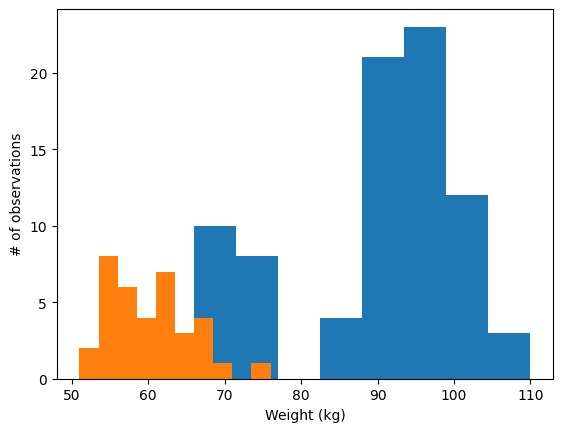
\includegraphics{../images/im242.png}
\end{frame}

\begin{frame}{``Step'' histogram}
\phantomsection\label{step-histogram}
Histograms allow us to see the distributions of the data in different
groups in our data.

In this exercise, you will select groups from the Summer 2016 Olympic
Games medalist dataset to compare the height of medalist athletes in two
different sports.
\end{frame}

\begin{frame}{``Step'' histogram}
\phantomsection\label{step-histogram-1}
The data is stored in a pandas DataFrame object called
summer\_2016\_medals that has a column ``Height''.

In addition, you are provided a pandas GroupBy object that has been
grouped by the sport.
\end{frame}

\begin{frame}{``Step'' histogram}
\phantomsection\label{step-histogram-2}
In this exercise, you will visualize and label the histograms of two
sports: ``Gymnastics'' and ``Rowing'' and see the marked difference
between medalists in these two sports.
\end{frame}

\begin{frame}[fragile]{``Step'' histogram}
\phantomsection\label{step-histogram-3}
\AddToHookNext{env/Highlighting/begin}{\tiny}

\begin{Shaded}
\begin{Highlighting}[]
\NormalTok{fig, ax }\OperatorTok{=}\NormalTok{ plt.subplots()}

\CommentTok{\# Plot a histogram of "Weight" for mens\_rowing}
\NormalTok{ax.hist(mens\_rowing[}\StringTok{"Weight"}\NormalTok{], histtype}\OperatorTok{=}\StringTok{\textquotesingle{}step\textquotesingle{}}\NormalTok{, label}\OperatorTok{=}\StringTok{"Rowing"}\NormalTok{, bins}\OperatorTok{=}\DecValTok{5}\NormalTok{)}
\CommentTok{\#\# (array([ 3., 18.,  4., 44., 15.]), array([ 55.,  66.,  77.,  88.,  99., 110.]), [\textless{}matplotlib.patches.Polygon object at 0x73f36d1f8d70\textgreater{}])}
\end{Highlighting}
\end{Shaded}
\end{frame}

\begin{frame}[fragile]{``Step'' histogram}
\phantomsection\label{step-histogram-4}
\AddToHookNext{env/Highlighting/begin}{\tiny}

\begin{Shaded}
\begin{Highlighting}[]
\CommentTok{\# Compare to histogram of "Weight" for mens\_gymnastics}
\NormalTok{ax.hist(mens\_gymnastics[}\StringTok{"Weight"}\NormalTok{], histtype}\OperatorTok{=}\StringTok{\textquotesingle{}step\textquotesingle{}}\NormalTok{, label}\OperatorTok{=}\StringTok{"Gymnastics"}\NormalTok{, bins}\OperatorTok{=}\DecValTok{5}\NormalTok{)}
\CommentTok{\#\# (array([10., 10., 10.,  5.,  1.]), array([51., 56., 61., 66., 71., 76.]), [\textless{}matplotlib.patches.Polygon object at 0x73f36d21b1a0\textgreater{}])}
\NormalTok{ax.set\_xlabel(}\StringTok{"Weight (kg)"}\NormalTok{)}
\NormalTok{ax.set\_ylabel(}\StringTok{"\# of observations"}\NormalTok{)}

\CommentTok{\# Add the legend and show the Figure}
\NormalTok{ax.legend()}
\NormalTok{plt.show()}
\end{Highlighting}
\end{Shaded}
\end{frame}

\begin{frame}{``Step'' histogram}
\phantomsection\label{step-histogram-5}
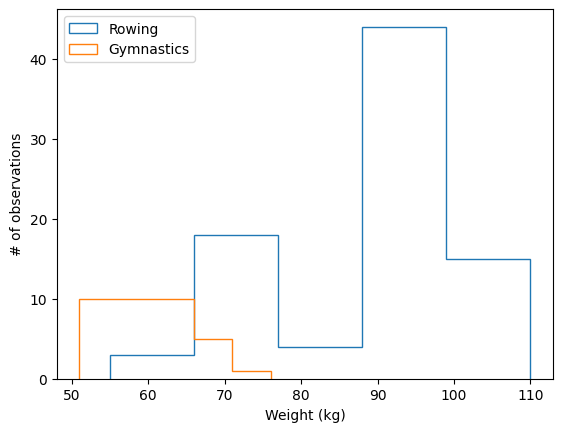
\includegraphics{../images/im243.png}
\end{frame}

\begin{frame}{Adding error-bars to a bar chart}
\phantomsection\label{adding-error-bars-to-a-bar-chart}
Statistical plotting techniques add quantitative information for
comparisons into the visualization.

For example, in this exercise, we will add error bars that quantify not
only the difference in the means of the height of medalists in the 2016
Olympic Games, but also the standard deviation of each of these groups,
as a way to assess whether the difference is substantial relative to the
variability within each group.
\end{frame}

\begin{frame}{Adding error-bars to a bar chart}
\phantomsection\label{adding-error-bars-to-a-bar-chart-1}
For the purpose of this exercise, you will have two DataFrames:
mens\_rowing holds data about the medalists in the rowing events and
mens\_gymnastics will hold information about the medalists in the
gymnastics events.
\end{frame}

\begin{frame}[fragile]{Adding error-bars to a bar chart}
\phantomsection\label{adding-error-bars-to-a-bar-chart-2}
\AddToHookNext{env/Highlighting/begin}{\tiny}

\begin{Shaded}
\begin{Highlighting}[]
\NormalTok{fig, ax }\OperatorTok{=}\NormalTok{ plt.subplots()}

\CommentTok{\# Add a bar for the rowing "Height" column mean/std}
\NormalTok{ax.bar(}\StringTok{"Rowing"}\NormalTok{, mens\_rowing[}\StringTok{"Height"}\NormalTok{].mean(), yerr}\OperatorTok{=}\NormalTok{mens\_rowing[}\StringTok{"Height"}\NormalTok{].std())}

\CommentTok{\# Add a bar for the gymnastics "Height" column mean/std}
\NormalTok{ax.bar(}\StringTok{"Gymnastics"}\NormalTok{, mens\_gymnastics[}\StringTok{"Height"}\NormalTok{].mean(), yerr}\OperatorTok{=}\NormalTok{mens\_gymnastics[}\StringTok{"Height"}\NormalTok{].std())}

\CommentTok{\# Label the y{-}axis}
\NormalTok{ax.set\_ylabel(}\StringTok{"Height (cm)"}\NormalTok{)}

\NormalTok{plt.show()}
\end{Highlighting}
\end{Shaded}
\end{frame}

\begin{frame}{Adding error-bars to a bar chart}
\phantomsection\label{adding-error-bars-to-a-bar-chart-3}
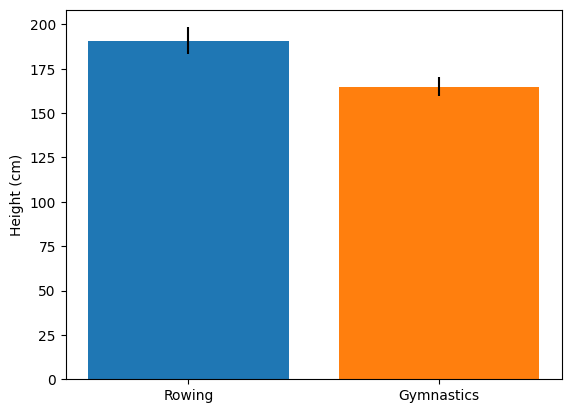
\includegraphics{../images/im244.png}
\end{frame}

\begin{frame}{Adding error-bars to a plot}
\phantomsection\label{adding-error-bars-to-a-plot}
Adding error-bars to a plot is done by using the errorbar method of the
Axes object.
\end{frame}

\begin{frame}{Adding error-bars to a plot}
\phantomsection\label{adding-error-bars-to-a-plot-1}
Here, you have two DataFrames loaded: seattle\_weather has data about
the weather in Seattle and austin\_weather has data about the weather in
Austin.

Each DataFrame has a column ``MONTH'' that has the names of the months,
a column ``MLY-TAVG-NORMAL'' that has the average temperature in each
month and a column ``MLY-TAVG-STDDEV'' that has the standard deviation
of the temperatures across years.
\end{frame}

\begin{frame}{Adding error-bars to a plot}
\phantomsection\label{adding-error-bars-to-a-plot-2}
In the exercise, you will plot the mean temperature across months and
add the standard deviation at each point as y errorbars.
\end{frame}

\begin{frame}[fragile]{Adding error-bars to a plot}
\phantomsection\label{adding-error-bars-to-a-plot-3}
\AddToHookNext{env/Highlighting/begin}{\tiny}

\begin{Shaded}
\begin{Highlighting}[]
\NormalTok{fig, ax }\OperatorTok{=}\NormalTok{ plt.subplots()}

\CommentTok{\# Add the Seattle temperature data in each month with standard deviation error bars}
\NormalTok{ax.errorbar(seattle\_weather[}\StringTok{"MONTH"}\NormalTok{], seattle\_weather[}\StringTok{"MLY{-}TAVG{-}NORMAL"}\NormalTok{], yerr}\OperatorTok{=}\NormalTok{seattle\_weather[}\StringTok{"MLY{-}TAVG{-}STDDEV"}\NormalTok{])}

\CommentTok{\# Add the Austin temperature data in each month with standard deviation error bars}
\NormalTok{ax.errorbar(austin\_weather[}\StringTok{"MONTH"}\NormalTok{], austin\_weather[}\StringTok{"MLY{-}TAVG{-}NORMAL"}\NormalTok{], yerr}\OperatorTok{=}\NormalTok{austin\_weather[}\StringTok{"MLY{-}TAVG{-}STDDEV"}\NormalTok{])}

\CommentTok{\# Set the y{-}axis label}
\NormalTok{ax.set\_ylabel(}\StringTok{"Temperature (Fahrenheit)"}\NormalTok{)}

\NormalTok{plt.show()}
\end{Highlighting}
\end{Shaded}
\end{frame}

\begin{frame}{Creating boxplots}
\phantomsection\label{creating-boxplots}
Boxplots provide additional information about the distribution of the
data that they represent.

They tell us what the median of the distribution is, what the
inter-quartile range is and also what the expected range of
approximately 99\% of the data should be. Outliers beyond this range are
particularly highlighted.
\end{frame}

\begin{frame}{Creating boxplots}
\phantomsection\label{creating-boxplots-1}
In this exercise, you will use the data about medalist heights that you
previously visualized as histograms, and as bar charts with error bars,
and you will visualize it as boxplots.
\end{frame}

\begin{frame}{Creating boxplots}
\phantomsection\label{creating-boxplots-2}
Again, you will have the mens\_rowing and mens\_gymnastics DataFrames
available to you, and both of these DataFrames have columns called
``Height'' that you will compare.
\end{frame}

\begin{frame}[fragile]{Creating boxplots}
\phantomsection\label{creating-boxplots-3}
\AddToHookNext{env/Highlighting/begin}{\tiny}

\begin{Shaded}
\begin{Highlighting}[]
\NormalTok{fig, ax }\OperatorTok{=}\NormalTok{ plt.subplots()}

\CommentTok{\# Add a boxplot for the "Height" column in the DataFrames}
\NormalTok{ax.boxplot([mens\_rowing[}\StringTok{"Height"}\NormalTok{], mens\_gymnastics[}\StringTok{"Height"}\NormalTok{]])}

\CommentTok{\# Add x{-}axis tick labels:}
\NormalTok{ax.set\_xticklabels([}\StringTok{"Rowing"}\NormalTok{, }\StringTok{"Gymnastics"}\NormalTok{])}

\CommentTok{\# Add a y{-}axis label}
\NormalTok{ax.set\_ylabel(}\StringTok{"Height (cm)"}\NormalTok{)}

\NormalTok{plt.show()}
\end{Highlighting}
\end{Shaded}
\end{frame}

\begin{frame}{Creating boxplots}
\phantomsection\label{creating-boxplots-4}
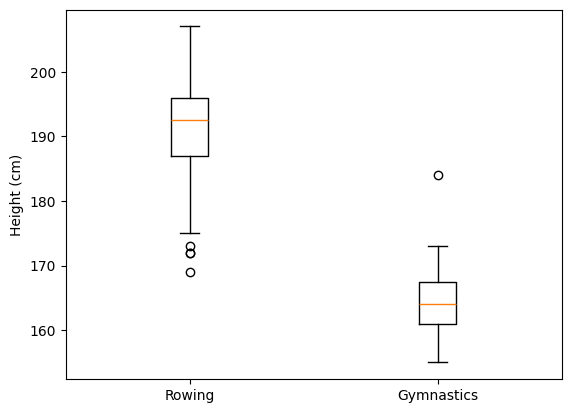
\includegraphics{../images/im246.png}
\end{frame}

\begin{frame}{Simple scatter plot}
\phantomsection\label{simple-scatter-plot}
Scatter are a bi-variate visualization technique. They plot each record
in the data as a point.

The location of each point is determined by the value of two variables:
the first variable determines the distance along the x-axis and the
second variable determines the height along the y-axis.
\end{frame}

\begin{frame}{Simple scatter plot}
\phantomsection\label{simple-scatter-plot-1}
In this exercise, you will create a scatter plot of the climate\_change
data.

This DataFrame, which is already loaded, has a column ``co2'' that
indicates the measurements of carbon dioxide every month and another
column, ``relative\_temp'' that indicates the temperature measured at
the same time.
\end{frame}

\begin{frame}[fragile]{Simple scatter plot}
\phantomsection\label{simple-scatter-plot-2}
\AddToHookNext{env/Highlighting/begin}{\tiny}

\begin{Shaded}
\begin{Highlighting}[]
\NormalTok{fig, ax }\OperatorTok{=}\NormalTok{ plt.subplots()}

\CommentTok{\# Add data: "co2" on x{-}axis, "relative\_temp" on y{-}axis}
\NormalTok{ax.scatter(climate\_change[}\StringTok{"co2"}\NormalTok{], climate\_change[}\StringTok{"relative\_temp"}\NormalTok{])}

\CommentTok{\# Set the x{-}axis label to "CO2 (ppm)"}
\NormalTok{ax.set\_xlabel(}\StringTok{"CO2 (ppm)"}\NormalTok{)}

\CommentTok{\# Set the y{-}axis label to "Relative temperature (C)"}
\NormalTok{ax.set\_ylabel(}\StringTok{"Relative temperature (C)"}\NormalTok{)}

\NormalTok{plt.show()}
\end{Highlighting}
\end{Shaded}
\end{frame}

\begin{frame}{Simple scatter plot}
\phantomsection\label{simple-scatter-plot-3}
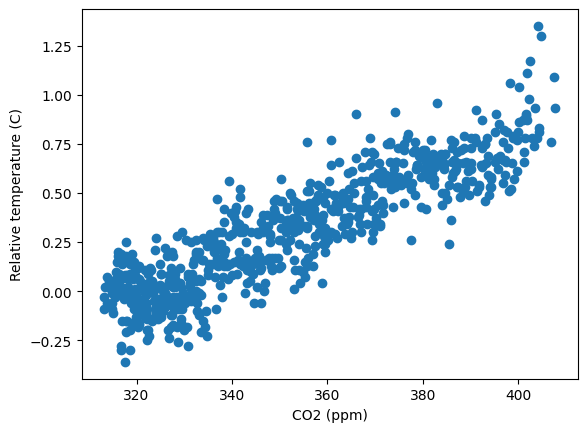
\includegraphics{../images/im247.png}
\end{frame}

\begin{frame}{Encoding time by color}
\phantomsection\label{encoding-time-by-color}
The screen only has two dimensions, but we can encode another dimension
in the scatter plot using color.

Here, we will visualize the climate\_change dataset, plotting a scatter
plot of the ``co2'' column, on the x-axis, against the
``relative\_temp'' column, on the y-axis.
\end{frame}

\begin{frame}{Encoding time by color}
\phantomsection\label{encoding-time-by-color-1}
We will encode time using the color dimension, with earlier times
appearing as darker shades of blue and later times appearing as brighter
shades of yellow.
\end{frame}

\begin{frame}[fragile]{Encoding time by color}
\phantomsection\label{encoding-time-by-color-2}
\AddToHookNext{env/Highlighting/begin}{\tiny}

\begin{Shaded}
\begin{Highlighting}[]
\NormalTok{fig, ax }\OperatorTok{=}\NormalTok{ plt.subplots()}

\CommentTok{\# Add data: "co2", "relative\_temp" as x{-}y, index as color}
\NormalTok{ax.scatter(climate\_change[}\StringTok{"co2"}\NormalTok{], climate\_change[}\StringTok{"relative\_temp"}\NormalTok{], c}\OperatorTok{=}\NormalTok{climate\_change.index)}

\CommentTok{\# Set the x{-}axis label to "CO2 (ppm)"}
\NormalTok{ax.set\_xlabel(}\StringTok{"CO2 (ppm)"}\NormalTok{)}

\CommentTok{\# Set the y{-}axis label to "Relative temperature (C)"}
\NormalTok{ax.set\_ylabel(}\StringTok{"Relative temperature (C)"}\NormalTok{)}

\NormalTok{plt.show()}
\end{Highlighting}
\end{Shaded}
\end{frame}

\begin{frame}{Encoding time by color}
\phantomsection\label{encoding-time-by-color-3}
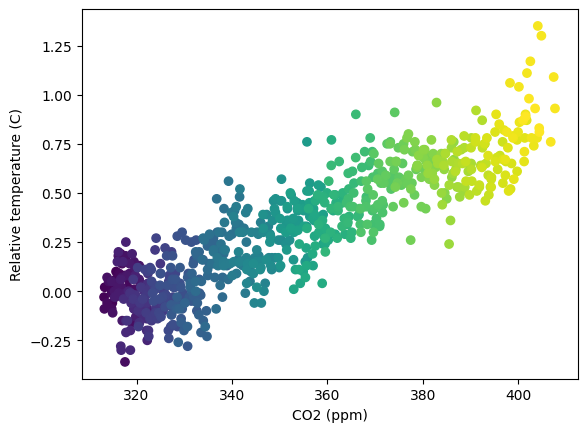
\includegraphics{../images/im248}
\end{frame}

\section{Sharing visualizations with
others}\label{sharing-visualizations-with-others}

\begin{frame}{Switching between styles}
\phantomsection\label{switching-between-styles}
Selecting a style to use affects all of the visualizations that are
created after this style is selected.

Here, you will practice plotting data in two different styles.
\end{frame}

\begin{frame}{Switching between styles}
\phantomsection\label{switching-between-styles-1}
The data you will use is the same weather data we used in the first
lesson: you will have available to you the DataFrame seattle\_weather
and the DataFrame austin\_weather, both with records of the average
temperature in every month.
\end{frame}

\begin{frame}[fragile]{Switching between styles}
\phantomsection\label{switching-between-styles-2}
\AddToHookNext{env/Highlighting/begin}{\tiny}

\begin{Shaded}
\begin{Highlighting}[]
\CommentTok{\# Use the "ggplot" style and create new Figure/Axes}
\NormalTok{plt.style.use(}\StringTok{\textquotesingle{}ggplot\textquotesingle{}}\NormalTok{)}
\NormalTok{fig, ax }\OperatorTok{=}\NormalTok{ plt.subplots()}
\NormalTok{ax.plot(seattle\_weather[}\StringTok{"MONTH"}\NormalTok{], seattle\_weather[}\StringTok{"MLY{-}TAVG{-}NORMAL"}\NormalTok{])}
\NormalTok{plt.show()}
\end{Highlighting}
\end{Shaded}
\end{frame}

\begin{frame}{Switching between styles}
\phantomsection\label{switching-between-styles-3}
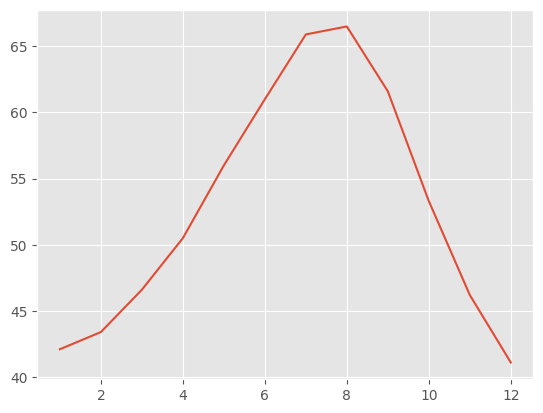
\includegraphics{../images/im249.png}
\end{frame}

\begin{frame}[fragile]{Switching between styles}
\phantomsection\label{switching-between-styles-4}
\AddToHookNext{env/Highlighting/begin}{\tiny}

\begin{Shaded}
\begin{Highlighting}[]
\CommentTok{\# Use the "Solarize\_Light2" style and create new Figure/Axes}
\NormalTok{plt.style.use(}\StringTok{\textquotesingle{}Solarize\_Light2\textquotesingle{}}\NormalTok{)}
\NormalTok{fig, ax }\OperatorTok{=}\NormalTok{ plt.subplots()}
\NormalTok{ax.plot(austin\_weather[}\StringTok{"MONTH"}\NormalTok{], austin\_weather[}\StringTok{"MLY{-}TAVG{-}NORMAL"}\NormalTok{])}
\NormalTok{plt.show()}
\end{Highlighting}
\end{Shaded}
\end{frame}

\begin{frame}{Switching between styles}
\phantomsection\label{switching-between-styles-5}
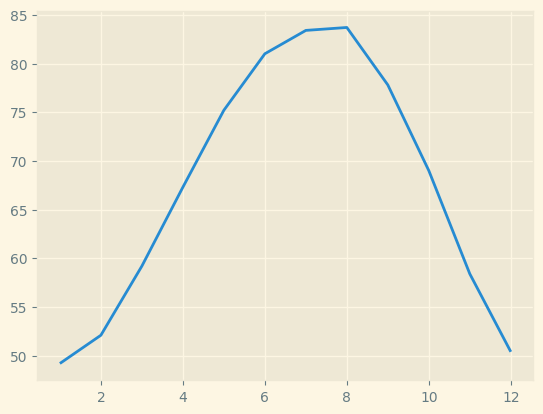
\includegraphics{../images/im250.png}
\end{frame}

\begin{frame}{Saving a file several times}
\phantomsection\label{saving-a-file-several-times}
If you want to share your visualizations with others, you will need to
save them into files. Matplotlib provides as way to do that, through the
savefig method of the Figure object.
\end{frame}

\begin{frame}{Saving a file several times}
\phantomsection\label{saving-a-file-several-times-1}
In this exercise, you will save a figure several times.

Each time setting the parameters to something slightly different.
\end{frame}

\begin{frame}[fragile]{Saving a file several times}
\phantomsection\label{saving-a-file-several-times-2}
\AddToHookNext{env/Highlighting/begin}{\tiny}

\begin{Shaded}
\begin{Highlighting}[]
\NormalTok{plt.style.use(}\StringTok{"default"}\NormalTok{)}
\NormalTok{fig, ax }\OperatorTok{=}\NormalTok{ plt.subplots()}
\NormalTok{ax.bar(medals.index, medals[}\StringTok{"Gold"}\NormalTok{])}
\NormalTok{ax.set\_xticklabels(medals.index, rotation}\OperatorTok{=}\DecValTok{90}\NormalTok{)}
\NormalTok{ax.set\_ylabel(}\StringTok{"Number of medals"}\NormalTok{)}

\CommentTok{\# Show the figure}
\NormalTok{plt.show()}
\end{Highlighting}
\end{Shaded}
\end{frame}

\begin{frame}{Saving a file several times}
\phantomsection\label{saving-a-file-several-times-3}
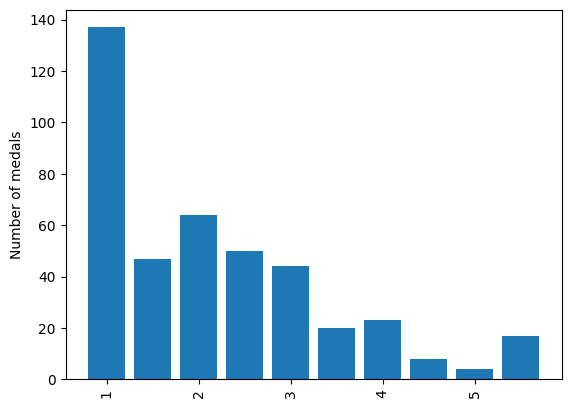
\includegraphics{../images/im251.png}
\end{frame}

\section{Save as a PNG file}\label{save-as-a-png-file}

\begin{frame}[fragile]{Save as a PNG file}
\phantomsection\label{save-as-a-png-file-1}
\AddToHookNext{env/Highlighting/begin}{\tiny}

\begin{Shaded}
\begin{Highlighting}[]
\NormalTok{fig.savefig(}\StringTok{\textquotesingle{}my\_figure.png\textquotesingle{}}\NormalTok{)}

\CommentTok{\# Save as a PNG file with 300 dpi}
\NormalTok{fig.savefig(}\StringTok{\textquotesingle{}my\_figure\_300dpi.png\textquotesingle{}}\NormalTok{, dpi}\OperatorTok{=}\DecValTok{300}\NormalTok{)}
\end{Highlighting}
\end{Shaded}
\end{frame}

\begin{frame}{Save a figure with different sizes}
\phantomsection\label{save-a-figure-with-different-sizes}
Before saving your visualization, you might want to also set the size
that the figure will have on the page.

To do so, you can use the Figure object's set\_size\_inches method. This
method takes a sequence of two values.
\end{frame}

\begin{frame}{Save a figure with different sizes}
\phantomsection\label{save-a-figure-with-different-sizes-1}
The first sets the width and the second sets the height of the figure.

Here, you will again have a Figure object called fig already provided
(you can run plt.show if you want to see its contents).
\end{frame}

\begin{frame}[fragile]{Save a figure with different sizes}
\phantomsection\label{save-a-figure-with-different-sizes-2}
\AddToHookNext{env/Highlighting/begin}{\tiny}

\begin{Shaded}
\begin{Highlighting}[]
\CommentTok{\# Set figure dimensions and save as a PNG}
\NormalTok{fig.set\_size\_inches([}\DecValTok{3}\NormalTok{, }\DecValTok{5}\NormalTok{])}
\NormalTok{fig.savefig(}\StringTok{\textquotesingle{}figure\_3\_5.png\textquotesingle{}}\NormalTok{)}
\CommentTok{\# Set figure dimensions and save as a PNG}
\NormalTok{fig.set\_size\_inches([}\DecValTok{5}\NormalTok{, }\DecValTok{3}\NormalTok{])}
\NormalTok{fig.savefig(}\StringTok{\textquotesingle{}figure\_5\_3.png\textquotesingle{}}\NormalTok{)}
\end{Highlighting}
\end{Shaded}
\end{frame}

\begin{frame}{Unique values of a column}
\phantomsection\label{unique-values-of-a-column}
One of the main strengths of Matplotlib is that it can be automated to
adapt to the data that it receives as input.

For example, if you receive data that has an unknown number of
categories, you can still create a bar plot that has bars for each
category.
\end{frame}

\begin{frame}{Unique values of a column}
\phantomsection\label{unique-values-of-a-column-1}
In this exercise and the next, you will be visualizing the weight of
athletes in the 2016 summer Olympic Games again, from a dataset that has
some unknown number of branches of sports in it.
\end{frame}

\begin{frame}{Unique values of a column}
\phantomsection\label{unique-values-of-a-column-2}
This will be loaded into memory as a pandas DataFrame object called
summer\_2016\_medals, which has a column called ``Sport'' that tells you
to which branch of sport each row corresponds.

There is also a ``Weight'' column that tells you the weight of each
athlete.

In this exercise, we will extract the unique values of the ``Sport''
column
\end{frame}

\begin{frame}[fragile]{Unique values of a column}
\phantomsection\label{unique-values-of-a-column-3}
\AddToHookNext{env/Highlighting/begin}{\tiny}

\begin{Shaded}
\begin{Highlighting}[]
\CommentTok{\# Extract the "Sport" column}
\NormalTok{sports\_column }\OperatorTok{=}\NormalTok{ summer\_2016\_medals[}\StringTok{"Sport"}\NormalTok{]}

\CommentTok{\# Find the unique values of the "Sport" column}
\NormalTok{sports }\OperatorTok{=}\NormalTok{ sports\_column.unique()}

\CommentTok{\# Print out the unique sports values}
\BuiltInTok{print}\NormalTok{(sports)}
\end{Highlighting}
\end{Shaded}
\end{frame}

\begin{frame}{Automate your visualization}
\phantomsection\label{automate-your-visualization}
One of the main strengths of Matplotlib is that it can be automated to
adapt to the data that it receives as input.

For example, if you receive data that has an unknown number of
categories, you can still create a bar plot that has bars for each
category.
\end{frame}

\begin{frame}{Automate your visualization}
\phantomsection\label{automate-your-visualization-1}
This is what you will do in this exercise.

You will be visualizing data about medal winners in the 2016 summer
Olympic Games again, but this time you will have a dataset that has some
unknown number of branches of sports in it.
\end{frame}

\begin{frame}{Automate your visualization}
\phantomsection\label{automate-your-visualization-2}
This will be loaded into memory as a pandas DataFrame object called
summer\_2016\_medals, which has a column called ``Sport'' that tells you
to which branch of sport each row corresponds.

There is also a ``Weight'' column that tells you the weight of each
athlete.
\end{frame}

\begin{frame}[fragile]{Automate your visualization}
\phantomsection\label{automate-your-visualization-3}
\AddToHookNext{env/Highlighting/begin}{\tiny}

\begin{Shaded}
\begin{Highlighting}[]
\NormalTok{fig, ax }\OperatorTok{=}\NormalTok{ plt.subplots()}

\CommentTok{\# Loop over the different sports branches}
\ControlFlowTok{for}\NormalTok{ sport }\KeywordTok{in}\NormalTok{ sports:}
  \CommentTok{\# Extract the rows only for this sport}
\NormalTok{  sport\_df }\OperatorTok{=}\NormalTok{ summer\_2016\_medals[summer\_2016\_medals[}\StringTok{"Sport"}\NormalTok{] }\OperatorTok{==}\NormalTok{ sport]}
  \CommentTok{\# Add a bar for the "Weight" mean with std y error bar}
\NormalTok{  ax.bar(sport, sport\_df[}\StringTok{"Weight"}\NormalTok{].mean(), yerr}\OperatorTok{=}\NormalTok{sport\_df[}\StringTok{"Weight"}\NormalTok{].std())}
\end{Highlighting}
\end{Shaded}
\end{frame}

\begin{frame}[fragile]{Automate your visualization}
\phantomsection\label{automate-your-visualization-4}
\AddToHookNext{env/Highlighting/begin}{\tiny}

\begin{Shaded}
\begin{Highlighting}[]
\NormalTok{ax.set\_ylabel(}\StringTok{"Weight"}\NormalTok{)}
\NormalTok{ax.set\_xticklabels(sports, rotation}\OperatorTok{=}\DecValTok{90}\NormalTok{)}

\CommentTok{\# Save the figure to file}
\NormalTok{fig.savefig(}\StringTok{"sports\_weights.png"}\NormalTok{)}
\end{Highlighting}
\end{Shaded}
\end{frame}

\begin{frame}{Automate your visualization}
\phantomsection\label{automate-your-visualization-5}
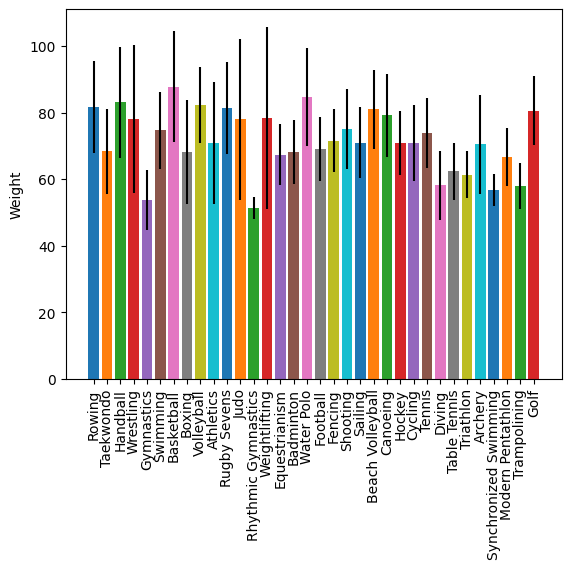
\includegraphics{../images/im252.png}
\end{frame}

\end{document}
